\section*{Organization of the appendix}

In \cref{sec:brownian} we remind the expression of the Brownian motion in local coordinates.
Details about the geodesic Brownian motion are given in \Cref{sec:geod-brown-moti}.
Background on the Skorokhod problem is given in \Cref{sec:refl-brown-moti}.
In \cref{sec:impl-score-match} we derive the implicit score matching loss.
We give details about the likelihood evaluation in \Cref{sec:likel-eval}.
Then in \cref{sec:time-revers-refl} we prove the time-reversal formula of reflected Brownian motion.

Additional results, training and miscellaneous experimental details are reported in \Cref{sec:exp_details}.

\section{Brownian motion in local coordinates}
\label{sec:brownian}

We consider a smooth function \(f \in \c{C}^\infty(\c{M})\).
The Laplace-Beltrami operator \(\Delta_\c{M}\) is given by \(\Delta_{\c{M}}(f) = \mathrm{div}(\mathrm{grad}(f)))\).
In local coordinates we have \begin{equation} { \mathrm{div}(X) = (\det(\mathfrak{g})^{-1/2}) \sum_{i=1}^d \partial_i (\det(\mathfrak{g})^{1/2} X_i) , } \end{equation} as well as \begin{equation} \mathrm{grad}(f) = \mathfrak{g}^{-1} \nabla f .
\end{equation}
Therefore, the Laplace-Beltrami operator is given by \begin{equation} { \Delta_\c{M}(f) = \sum_{i,j=1}^d \mathfrak{g}_{i,j}^{-1} \partial_{i,j} f + (\det(\mathfrak{g})^{-1/2}) \sum_{i,j=1}^d \partial_i (\det(\mathfrak{g})^{1/2} \mathfrak{g}_{i,j}^{-1}) \partial_j f .
	}
\end{equation}
Therefore, in local coordinates the infinitesimal generator associated with the Laplace-Beltrami operator is given by \begin{equation} { \mathcal{A}(f) = \sum_{i,j=1}^d \mathfrak{g}_{i,j}^{-1} \partial_{i,j} f + \langle b^i, \nabla f \rangle ,} \end{equation} with \begin{equation} \label{eq:def_drift} { b^i = (\det(\mathfrak{g})^{-1/2}) \sum_{j=1}^d \partial_j (\det(\mathfrak{g})^{1/2} \mathfrak{g}_{i,j}^{-1}) .
	}
\end{equation}
Therefore, the dual operator associated with \(\mathcal{A}\) is given by \begin{equation} { \mathcal{A}^\star(f) = \sum_{i,j=1}^d \partial_{i,j} (\mathfrak{g}_{i,j}^{-1} f) - \sum_{i=1}^d \partial_i (b^i f) .
	}
\end{equation}
Note that by letting \(f = \det(\mathfrak{g})^{1/2}\) we get that \(\mathcal{A}^\star(f) = 0\) and therefore we recover that \(p \propto \det(\mathfrak{g})\) is the invariant distribution of the Brownian motion.

\paragraph{Langevin dynamics on \(\c{M}\).}
We know that the Brownian motion targets \( \det(\mathfrak{g})^{1/2}\).
Therefore in order to correct and sample from the uniform distribution we consider the Langevin dynamics \begin{equation} \mathrm{d} \v{X}_t = -\mathrm{grad} \log (\det(\mathfrak{g})^{1/2})(\v{X}_t) \mathrm{d} t + \sqrt{2} \mathrm{d} \v{B}_t^\c{M} .
\end{equation}
Note that in the previous equation \(\mathrm{grad}\) and \(\v{B}_t^{\c{M}}\) are defined with respect to.
the metric of the manifold.
In local coordinates we have \begin{equation} \label{eq:forward_process} \mathrm{d} \v{X}_t = \{b -\mathrm{grad} \log (\det(\mathfrak{g})^{1/2})\}(\v{X}_t) \mathrm{d} t + \sqrt{2} \mathfrak{g}(\v{X}_t)^{-1/2} \mathrm{d} \v{B}_t .
\end{equation}
where \(b = \{b^i\}_{i=1}^d\) is given in \eqref{eq:def_drift}.
In addition, we have \begin{equation} \label{eq:expansion_grad} \mathrm{grad} \log (\det(\mathfrak{g})^{1/2}) = \det(\mathfrak{g})^{-1/2} \mathfrak{g}^{-1} \nabla \det(\mathfrak{g}) .
\end{equation}
Using \eqref{eq:def_drift} we have \begin{equation} b^i = {(\det(\mathfrak{g})^{-1/2}) \sum_{j=1}^d \partial_j (\det(\mathfrak{g})^{1/2} \mathfrak{g}_{i,j}^{-1})} = {\sum_{j=1}^d \partial_j \mathfrak{g}_{i,j}^{-1} + \mathrm{grad} \log (\det(\mathfrak{g})^{1/2})_i} \end{equation} This can also be rewritten as \begin{equation} \mathrm{div}_\c{M}(\mathfrak{g}^{-1}) = {\mu + \mathrm{grad} \log (\det(\mathfrak{g})^{1/2}) ,} \end{equation} with \begin{equation} {\mu_i = \sum_{j=1}^d \partial_j \mathfrak{g}_{i,j}^{-1} .
	}
\end{equation}
Combining this result and \eqref{eq:expansion_grad} we get that \eqref{eq:forward_process} can be rewritten as \begin{equation} \mathrm{d} \v{X}_t = \mu(\v{X}_t) + \sqrt{2} \mathrm{d} \v{B}_t .
\end{equation}
Note that (up to a factor \(2\)) this is the same SDE as the one considered in \textcite{lee2017Geodesic}.

\section{Geodesic Brownian Motion}
\label{sec:geod-brown-moti}

In this section, we provide some details on the geodesics Brownian motion introduced in \Cref{sec:bsgm}.
In the rest of the section, we make the following assumption.

\begin{assumption}
	\label{assum:log_barrier_method}
	\(\cl{\c{M}} \subset \R^d\) is compact and
	\(\mathfrak{g}^{-1}: \ \c{M} \to \mathcal{S}_d^{++}\) can be
	\(\mathrm{C}^\infty(\R^d, \R^{d \times d})\).
\end{assumption}

First, we start by showing that the process \((\v{X}_t)_{t \geq 0}\) defined in \eqref{eq:langevin_hessian_manifold} exists and that we have for any \(t \geq 0\), \(\v{X}_t \in \c{M}\).
We recall that \(\mathfrak{g} = \nabla^2 \phi\) and \(\lim_{x \to \partial \c{M}} \Phi(x) = +\infty\).

\begin{proposition}
	Assume \textup{\Cref{assum:log_barrier_method}}.
	For any \(x_0 \in \c{M}\), there exists a unique strong solution to \eqref{eq:langevin_hessian_manifold} denoted \((\v{X}_t)_{t \geq 0}\).
	In addition, we have that for any \(t \geq 0\), \(\v{X}_t \in \c{M}\) almost surely.
	More precisely, we have \(\E\sbr{\phi(\v{X}_t)} \leq \phi(x_0) + t\).
\end{proposition}

\begin{proof}
	A unique strong solution \((\v{X}_t)_{t \geq 0}\) of \eqref{eq:langevin_hessian_manifold} with starting point \(x_0\in \c{M}\) exists since the coefficients are smooth, see \cite[Theorem 3.1, p.165]{ikeda2014stochastic}.
	For any \(A \geq 0\), we define \(\tau_A = \inf \cbr{t \geq 0 \; : \; \Phi(\v{X}_t) \geq A}\).
	Note that for any \(t \in \cbr{0, \tau_A}\), \(\Phi(\v{X}_t) \in \c{M}\).
	Using It\^o formula, we have for any \(t \geq 0\) \begin{equation}  \E\sbr{\Phi(\v{X}_{t \wedge \tau_A})} = \Phi(x_0) + \E\sbr{\int_0^{t \wedge \tau_A} \mathrm{Tr}(\mathfrak{g}^{-1}(\v{X}_s) \nabla^2 \Phi(\v{X}_s) )\mathrm{d} s} = \Phi(x_0) + \E\sbr{t \wedge \tau_A} .
	\end{equation}
	Using Fatou's lemma, and letting \(A \to +\infty\), we conclude the proof.
\end{proof}

In the next result, we show that the uniform distribution is the \emph{unique} invariant probability distribution for \((\v{X}_t)_{t \geq 0}\) and that \((\v{X}_t)_{t \geq 0}\) converges to this invariant distribution.
We refer to \cite[Section 2, p.490]{meyn1993stability} for a definition of irreducibility.
We recall that the total variation of a finite (not necessarily non-negative) measure \(\mu\) over \(\R^d\) is given by \(\| \mu \|_{\mathrm{TV}} = \sup \cbr{\mu(\mathsf{A}) \; : \; \mathsf{A} \in \c{B}(\R^d)}\).

\begin{proposition}
	Assume \textup{\Cref{assum:log_barrier_method}}.
	\((\v{X}_t)_{t \geq 0}\) is
	\(\pi\)-irreducible, the uniform distribution over \(\c{M}\) is the only invariant
	probability distribution and
	\(\lim_{t \to +\infty} \|\mathrm{P}_t - \pi\|_{\mathrm{TV}} = 0\), where \(\mathrm{P}_t\) is
	the distribution of \(\v{X}_t\) for any \(t \geq 0\) and \(\pi\) is the uniform
	distribution over \(\c{M}\).
\end{proposition}

\begin{proof}
	Since \(x \mapsto \mathrm{div}(\mathfrak{g}^{-1})(x)\) and \(x \mapsto \mathfrak{g}^{-1}\) are smooth and \(\mathfrak{g}^{-1}(x)\) is positive definite for any \(x \in \c{M}\), we have that \((\v{X}_t)_{t \geq 0}\) is \(\pi\)-irreducible, extending \cite[Lemma 1.4]{bhattacharya1978criteria} to \(\c{M}\) and using \cite[Proposition 2.1]{meyn1993stability}.
	In addition, \((\v{X}_t)_{t \geq 0}\) is \(\mathrm{T}\)-Feller using \cite[Proposition 3.3]{meyn1993stability}.
	Combining these results and the fact that \(\c{M}\) is bound, we get that \((\v{X}_t)_{t \geq 0}\) is positive Harris recurrent \cite[Theorem 3.2]{meyn1993stability}.
	The uniform distribution \(\pi\) is an invariant distribution for \eqref{eq:langevin_hessian_manifold}.
	Since \((\v{X}_t)_{t \geq 0}\) is \(\pi\)-irreducible, we get that this invariant measure is unique.
	Hence, we conclude using \cite[Theorem 6.1]{meyn1993stability}.
\end{proof}

Note that the convergence result in total variation could be improved.
In particular, quantitative geometric results could be derived.
We finish this section, by applying results from the Malliavin calculus to show that for any \(t > 0\), \(\v{X}_t\) admits a density with respect to.
the Lebesgue measure.

\begin{proposition}
	Assume \textup{\Cref{assum:log_barrier_method}}.
	Then, for any \(t \geq 0\), \(\v{X}_t\) admits a smooth density \(p_t\) with respect to.
	the Lebesgue measure.
\end{proposition}

\begin{proof}
	This is a direct consequence of \cite[Theorem 2.3.3]{nualart2006malliavin}.
\end{proof}

\section{Reflected Brownian Motion and Skorokhod problems}
\label{sec:refl-brown-moti}

In this section, we provide the basic definitions and results to derive the time-reversal of the reflected Brownian motion in \Cref{sec:time-revers-refl}.
We follow closely the presentation of \cite{lions1984stochastic} and \cite{burdzy2004heat}.
We first define the \emph{Skorokhod problem} for deterministic problems.
We consider \(\c{M}\) to be a smooth open bounded domain.
We recall that the normal vector \(n\) is defined on \(\partial \c{M}\) and we set \(n(x) = 0\) for any \(x \notin \partial \c{M}\).

Before giving the definition of the \emph{Skorokhod problem}, we recall what is the space of functions of \emph{bounded variations}.

\begin{definition}
	Let \(a, b \in \del{-\infty, +\infty}\) and \(f: \in \mathrm{C}(\cbr{a,b}, \R)\).
	We define the \emph{total variation} of \(f\) as \begin{equation}  \mathrm{V}_{a,b}(f) = \sup \cbr{\sum_{i=0}^{n-1} \norm{f(x_{i+1}) - f(x_i)} \; : \; (x_i)_{i=0}^{n-1}, \ a=x_0 \leq \dots \leq x_n = b, \ n \in \N} .
	\end{equation}
	\(f\) has bounded variations over \(\cbr{a,b}\) if
	\(\mathrm{V}_{a,b}(f) < +\infty\).
	Let \(f \in \mathrm{C}(\cobr{0,+\infty}, \R)\).
	\(f\) has bounded variations over \(\cobr{0,+\infty}\) if for any
	\(b>0\), \(f\) has bounded variations over \(\cbr{0,b}\).
\end{definition}

The notion of bounded variation is a relaxation of the differentiability requirement.
In particular, if \(f \in \mathrm{C}^1(\cbr{a,b}, \R)\), we have \(\mathrm{V}_{a,b}(f) = \int_a^b \norm{f'(t)} \mathrm{d} t\).
In the definition of the \emph{Skorokhod problem}, we will see that this relaxation is necessary, even in the deterministic setting.

For any function of bounded variation \(f \in \mathrm{C}(\cbr{a,b}, \R)\) on \(\cbr{a,b}\), we define \(\abs{f}: \ \cbr{a,b} \to \cobr{0,+\infty}\) given for any \(t \in \cbr{a,b}\) by \(\abs{f}_t = \mathrm{V}_{a,t}(f)\).
Note that \(\abs{f}\) is non-decreasing and right-continuous.
Therefore, we can define the measure \(\mu_{\abs{f}}\) on \(\cbr{a,b}\), given for any \(s, t \in \cbr{a,b}\) with \(t \geq s\) by \(\mu_{\abs{f}}([s,t]) = \abs{f}(t) - \abs{f}(s)\).
In particular, for any \(\varphi: \cbr{a,b} \to \R_+\), we define \begin{equation}  \int_a^b \varphi(t) \mathrm{d} \abs{f}_t = \int_a^b \varphi(t) \mathrm{d} \mu_{\abs{f}}(t) .
\end{equation}
In addition, \(f\) can be decomposed in a difference of two non-decreasing processes right continuous processes \(g_1\), \(g_2\), where for any \(t \in \cbr{a,b}\), \(f(t) = g_1(t) - g_2(t)\), \(g_1(t) = \abs{f}_t\) and \(g_2(t) = \abs{f}_t - f(t)\).
Hence, for every \(\varphi\) bounded on \(\cbr{a,b}\), we can define \begin{equation}  \int_a^b \varphi(t) \mathrm{d} f(t) = \int_a^b \varphi(t) \mathrm{d} g_1(t) - \int_a^b \varphi(t) \mathrm{d} g_2(t) .
\end{equation}
Note that these definitions can be extended to the setting where \(f: \ \cbr{a,b} \to \R^d\).

We begin with the following result, see \cite{lions1984stochastic}.

\begin{theorem}
	\label{thm:existence_reflected_det}
	Let \((x_t)_{t \geq 0} \in \mathrm{C}(\cobr{0, +\infty}, \R)\).
	Then, there exists a unique couple \((\bar{x}_t, k_t)_{t \geq 0}\) such that \begin{enumerate}[label=(\alph*)] \item \((k_t)_{t \geq 0}\) has bounded variation over \(\cobr{0,+\infty}\).
		\item \((\bar{x}_t)_{t \geq 0} \in \mathrm{C}(\cobr{0,+\infty}, \cl{\c{M}})\).
		\item For any \(t \geq 0\), \(x_t + k_t = \bar{x}_t\). \label{item:decomp}
		\item For any \(t \geq 0\),
		      \(\abs{k}_t = \int_0^t \mathbf{1}_{\bar{x}_s \in \partial \c{M}}(\bar{x}_s) \mathrm{d} \abs{k}_s\) and
		      \(k_t = \int_0^t n(\bar{x}_s) \mathrm{d} \abs{k}_s\).
	\end{enumerate}
\end{theorem}

Let us discuss \Cref{thm:existence_reflected_det}.
First, \Cref{thm:existence_reflected_det}-\ref{item:decomp} states the original (unconstrained) process \((x_t)_{t \geq 0}\) can be decomposed into a constrained version \((\bar{x}_t)_{t \geq 0}\) and a bounded variation process \((k_t)_{t \geq 0}\).
The process \((\abs{k}_t)_{t \geq 0}\) counts the number of times the constrained process \((\bar{x}_t)_{t \geq 0}\) hits the boundary.
More formally, we have \(\abs{k}_t = \int_0^t \mathbf{1}_{x \in \partial \c{M}}(\bar{x}_s) \mathrm{d} \abs{k}_s\).
When, we hit the boundary, we reflect the process.
This condition is expressed in \(k_t = \int_0^t n(\bar{x}_s) \mathrm{d} \abs{k}_s\).

We now consider the extension to stochastic processes.
We are given \((\v{X}_t)_{t \geq 0}\) such that \begin{equation} \label{eq:sde} \mathrm{d} \v{X}_t = b(\v{X}_t) \mathrm{d} t + \sigma(t) \mathrm{d} \v{B}_t , \end{equation} where \((\v{B}_t)_{t \geq 0}\) is a \(d\)-dimensional Brownian motion.
We also assume that \(b\) and \(\sigma\) are Lipschitz which implies the existence and strong uniqueness of \((\v{X}_t)_{t \geq 0}\).
We have the following result \cite{lions1984stochastic}.

\begin{theorem}
	\label{thm:existence_reflected_sto}
	There exists a unique process \((\bar{\v{X}}_t, \v{k}_t)_{t \geq 0}\) such that \begin{enumerate}[label=(\alph*)] \item \((\v{k}_t)_{t \geq 0}\) has bounded variation over \(\cobr{0,+\infty}\) almost surely.
		\item \((\bar{\v{X}}_t)_{t \geq 0} \in \mathrm{C}(\cobr{0,+\infty}, \cl{\c{M}})\).
		\item For any \(t \geq 0\), \(\bar{\v{X}}_t = \bar{\v{X}}_0 + \int_0^t b(\bar{\v{X}}_s) \mathrm{d} s + \int_0^t \sigma(\bar{\v{X}}_s) \mathrm{d} \v{B}_s - \v{k}_t\). \label{item:sde_ref}
		\item For any \(t \geq 0\),
		      \(\abs{\v{k}}_t = \int_0^t \mathbf{1}_{\bar{x}_s \in \partial \c{M}}(\bar{x}_s) \mathrm{d} \abs{\v{k}}_s\) and
		      \(\v{k}_t = \int_0^t n(\bar{x}_s) \mathrm{d} \abs{\v{k}}_s\).
	\end{enumerate}
\end{theorem}

The process \((\v{X}_t)_{t \geq 0}\) is almost surely continuous, so we could apply the previous theorem almost surely for all the realizations of the process,.
However, this does not tell us if the obtained solutions \((\bar{\v{X}}_t, \v{k}_t)_{t \geq 0}\) form themselves a process.
The main difference with \Cref{thm:existence_reflected_det} is in \Cref{thm:existence_reflected_sto}-\ref{item:sde_ref} which differs from \Cref{thm:existence_reflected_sto}-\ref{item:decomp}.
Note that in the case where \(b=0\) and \(\sigma =\m{I}\) we recover \Cref{thm:existence_reflected_sto}-\ref{item:decomp}.
This is not true in the general case.
However, it can be seen that for any realization of the process \((\bar{\v{X}}_t)_{t \geq 0}\), we have that \((\bar{\v{X}}_t, \v{k}_t)_{t \geq 0}\) is solution of the \emph{deterministic} Skorokhod problem by letting \(x_t = \bar{\v{X}}_0 + \int_0^t b(\bar{\v{X}}_s) \mathrm{d} s + \int_0^t \sigma(\bar{\v{X}}_s) \mathrm{d} \v{B}_s\).
The backward and forward Kolmogorov equations can be found in \cite{burdzy2004heat}.
Note that the presence of the process \((\v{k}_t)_{t \geq 0}\) incurs notable complications compared to unconstrained processes.
In particular, there is no martingale problem associated with weak solutions of reflected SDEs but only sub-martingale problems, see \cite{kang2017submartingale} for instance.

\section{Implicit Score Matching Loss}
\label{sec:impl-score-match}

\subsection{Proof of ISM}
\label{app:proof_for_ism}

Using the divergence theorem, we have 
\begin{align} \label{eq:score_matching_app} 
		& {(1/2) \int_\c{M} \| \mathbf{s}_{t, \theta}(x) - \nabla \log p_t(x) \|^2 p_t(x) \mathrm{d} \mu(x)} \\ 
		& = (1/2) \int_\c{M} \| \mathbf{s}_{t, \theta}(x) \|^2 p_t(x) \mathrm{d} \mu(x)  - \int_\c{M} \langle \mathbf{s}_{t, \theta}(x), \nabla \log p_t(x) \rangle p_t(x) \mathrm{d} \mu(x) \\
		&\qquad + (1/2) \int_\c{M} \| \nabla \log p_t(x) \|^2 p_t(x) \mathrm{d} \mu(x) \\
		& = {(1/2) \int_\c{M} \| \mathbf{s}_{t, \theta}(x) \|^2 p_t(x) \mathrm{d} \mu(x) -\int_{\partial \c{M}} \langle \mathbf{s}_{t, \theta}(x), \mathbf{n} \rangle p_t(x) \mathrm{d} \nu(x)} \\
		& \qquad + \int_\c{M} \mathrm{div}(\mathbf{s}_{t, \theta})(x) p_t(x) \mathrm{d} \mu(x) + (1/2) \int_\c{M} \| \nabla \log p_t(x) \|^2 p_t(x) \mathrm{d} \mu(x).
\end{align}
Using that \(\innerprod{\mathbf{s}_{t, \theta}(x)}{\v{n}(x)} = 0\) for all \(x \in \partial\c{M}\), we get that 
\begin{align} & {(1/2) \int_\c{M} \| \mathbf{s}_{t, \theta}(x) - \nabla \log p_t(x) \|^2 p_t(x) \mathrm{d} \mu(x)} \\ 
	& \qquad = {(1/2) \int_\c{M} \| \mathbf{s}_{t, \theta}(x) \|^2 p_t(x) \mathrm{d} \mu(x)}  \\ 
	&\qquad \qquad + \int_\c{M} \mathrm{div}(\mathbf{s}_{t, \theta})(x) p_t(x) \mathrm{d} \mu(x) + (1/2) \int_\c{M} \| \nabla \log p_t(x) \|^2 p_t(x) \mathrm{d} \mu(x), 
\end{align} which concludes the proof.

\subsection{Importance of scaling function}\label{sec:boundary_score}

As discussed in \Cref{sec:score-netw-param}, we include a monotone scaling function \(h\) which is zero close to the boundary to ensure the relevant conditions are met for the score matching loss and the boundary conditions.
This may seem like a technical detail, but is of significant practical importance.
Upon removal of the scaling function, we observe that the learned score functions behave strangely around the boundary in the reverse process, leading to samples that do not match the forward process.
The problems are apparent when comparing the top three plots of Fig.
\ref{fig:no_scaling} and Fig. \ref{fig:scaling}.
Interestingly, we found that these issues early on in the sampling are smoothed out by the end of the reverse process, but still lead to a failure to recover the target density.

\begin{figure}[H]
	\centering
	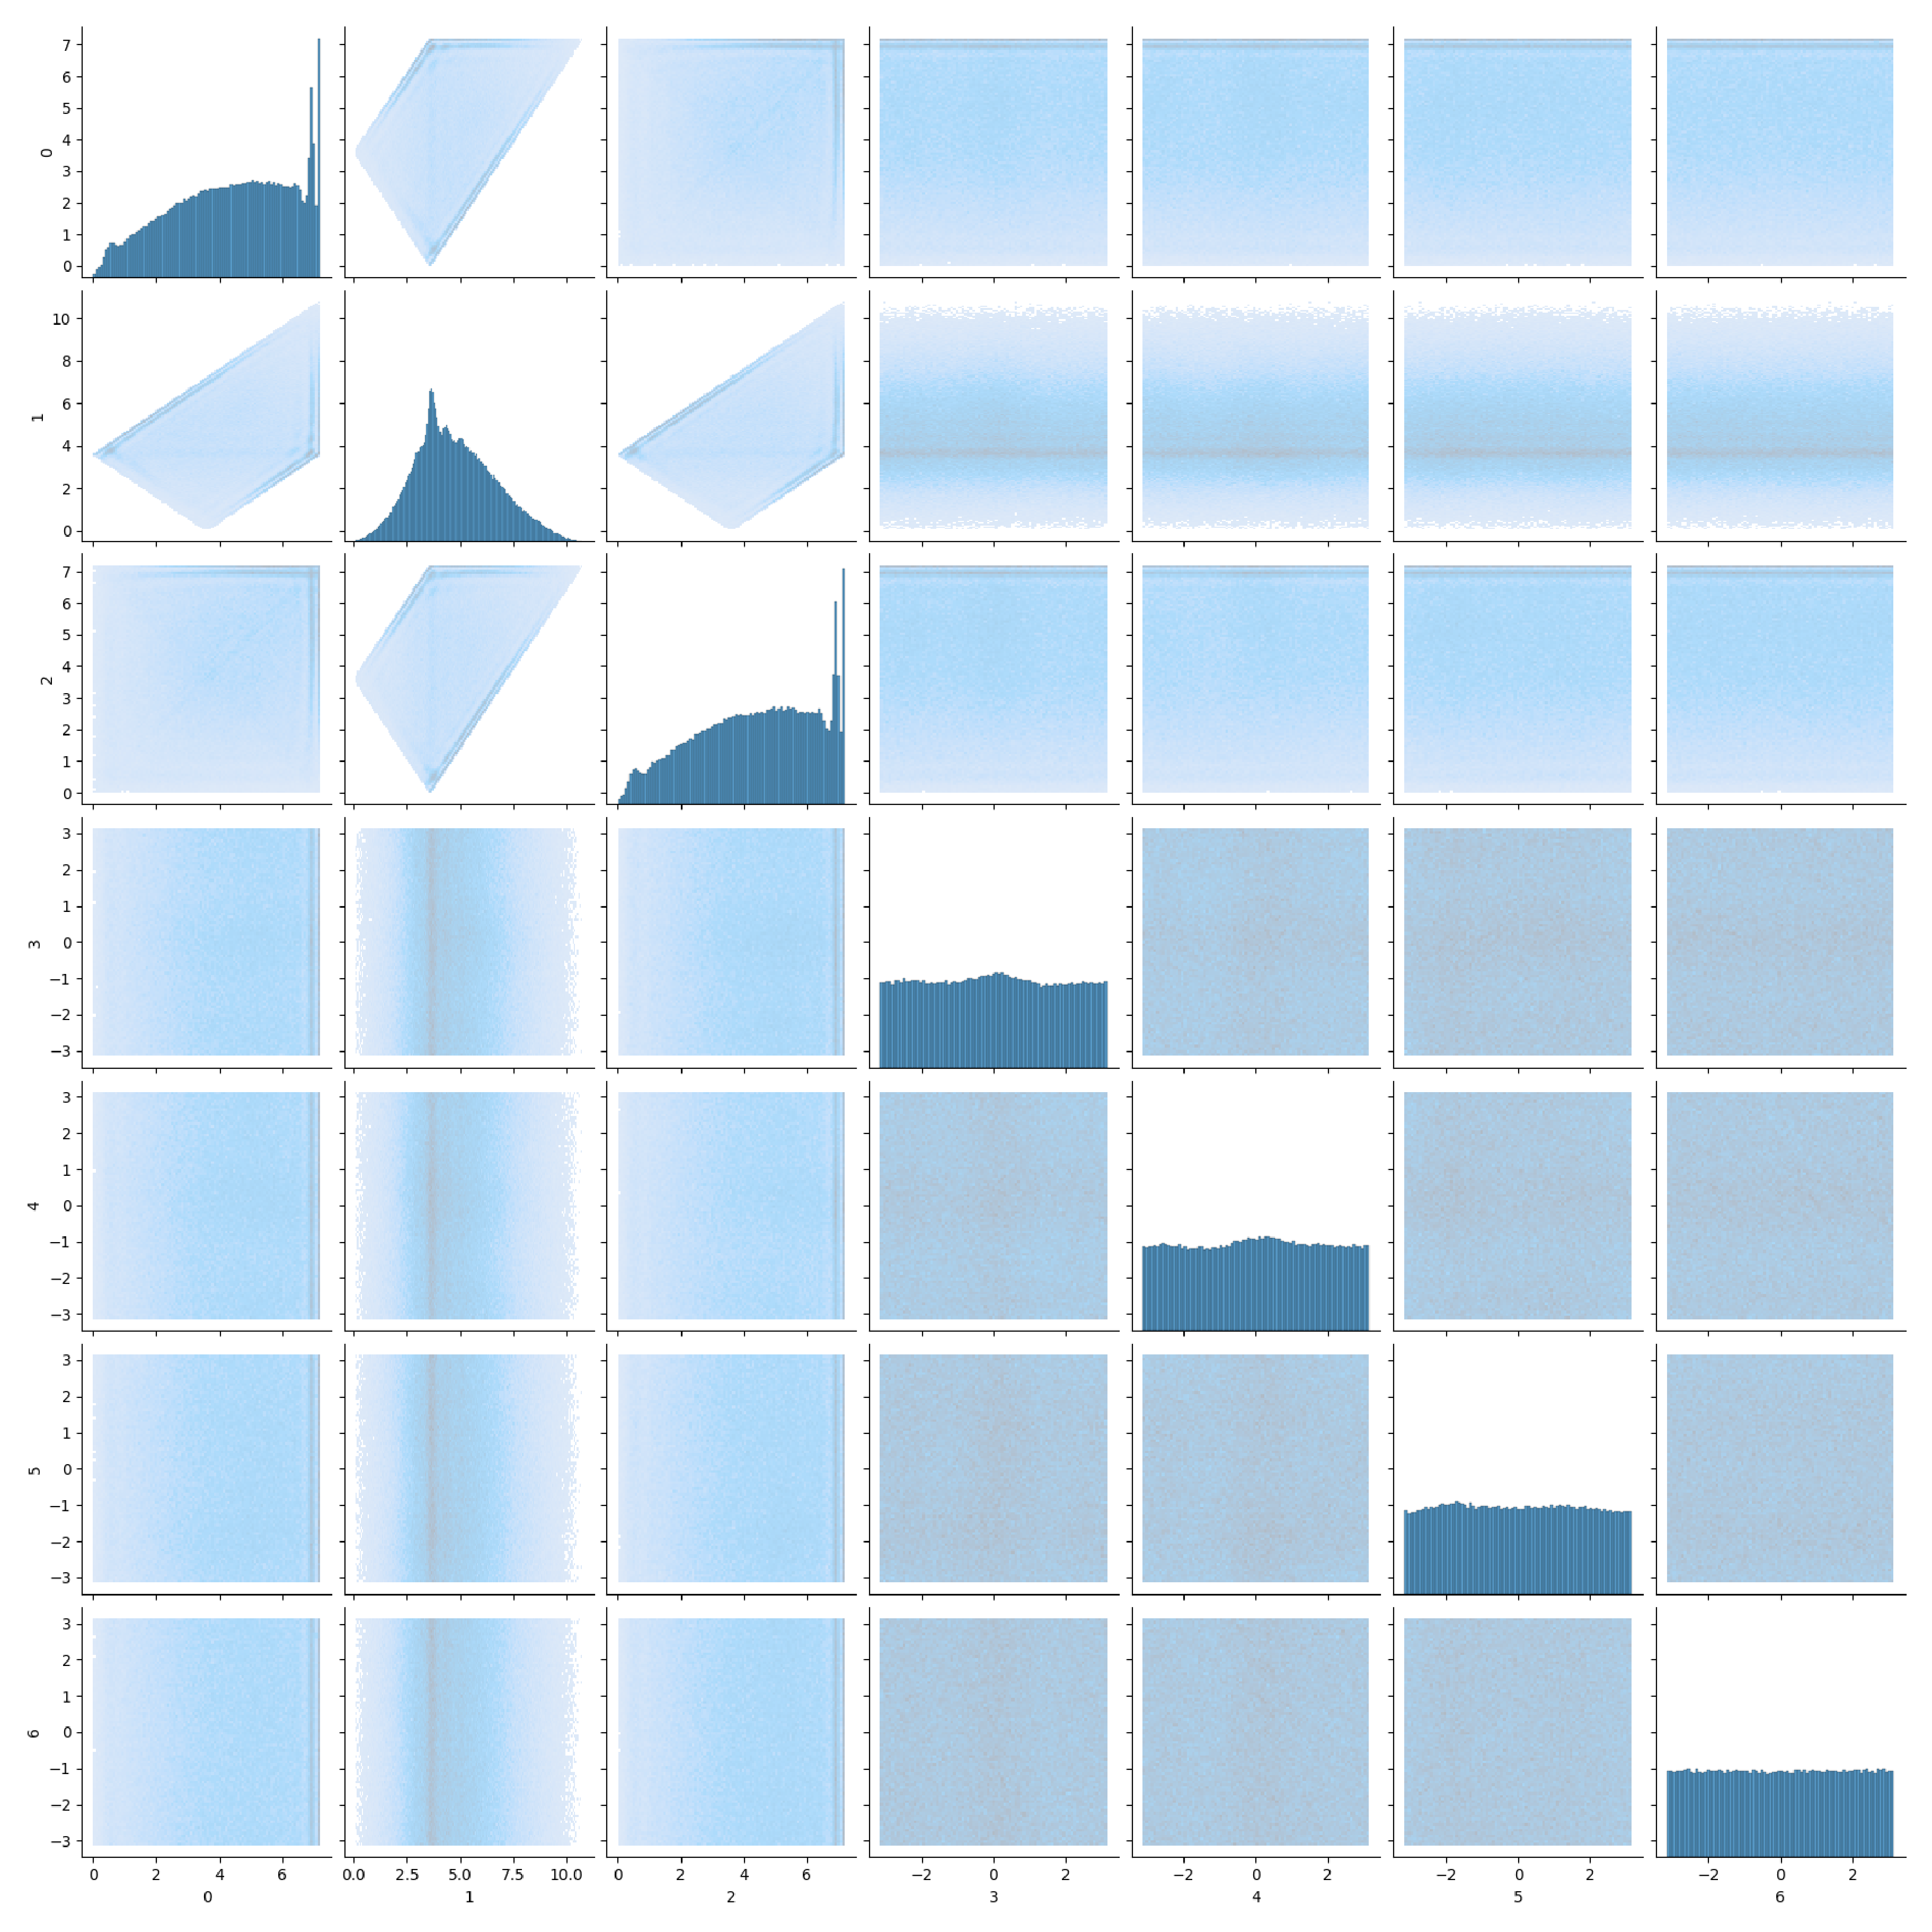
\includegraphics[width=0.4\textwidth]{images/constrained_diffusion/Positive Boundary, Backward Sampling, t=0.9.pdf}
	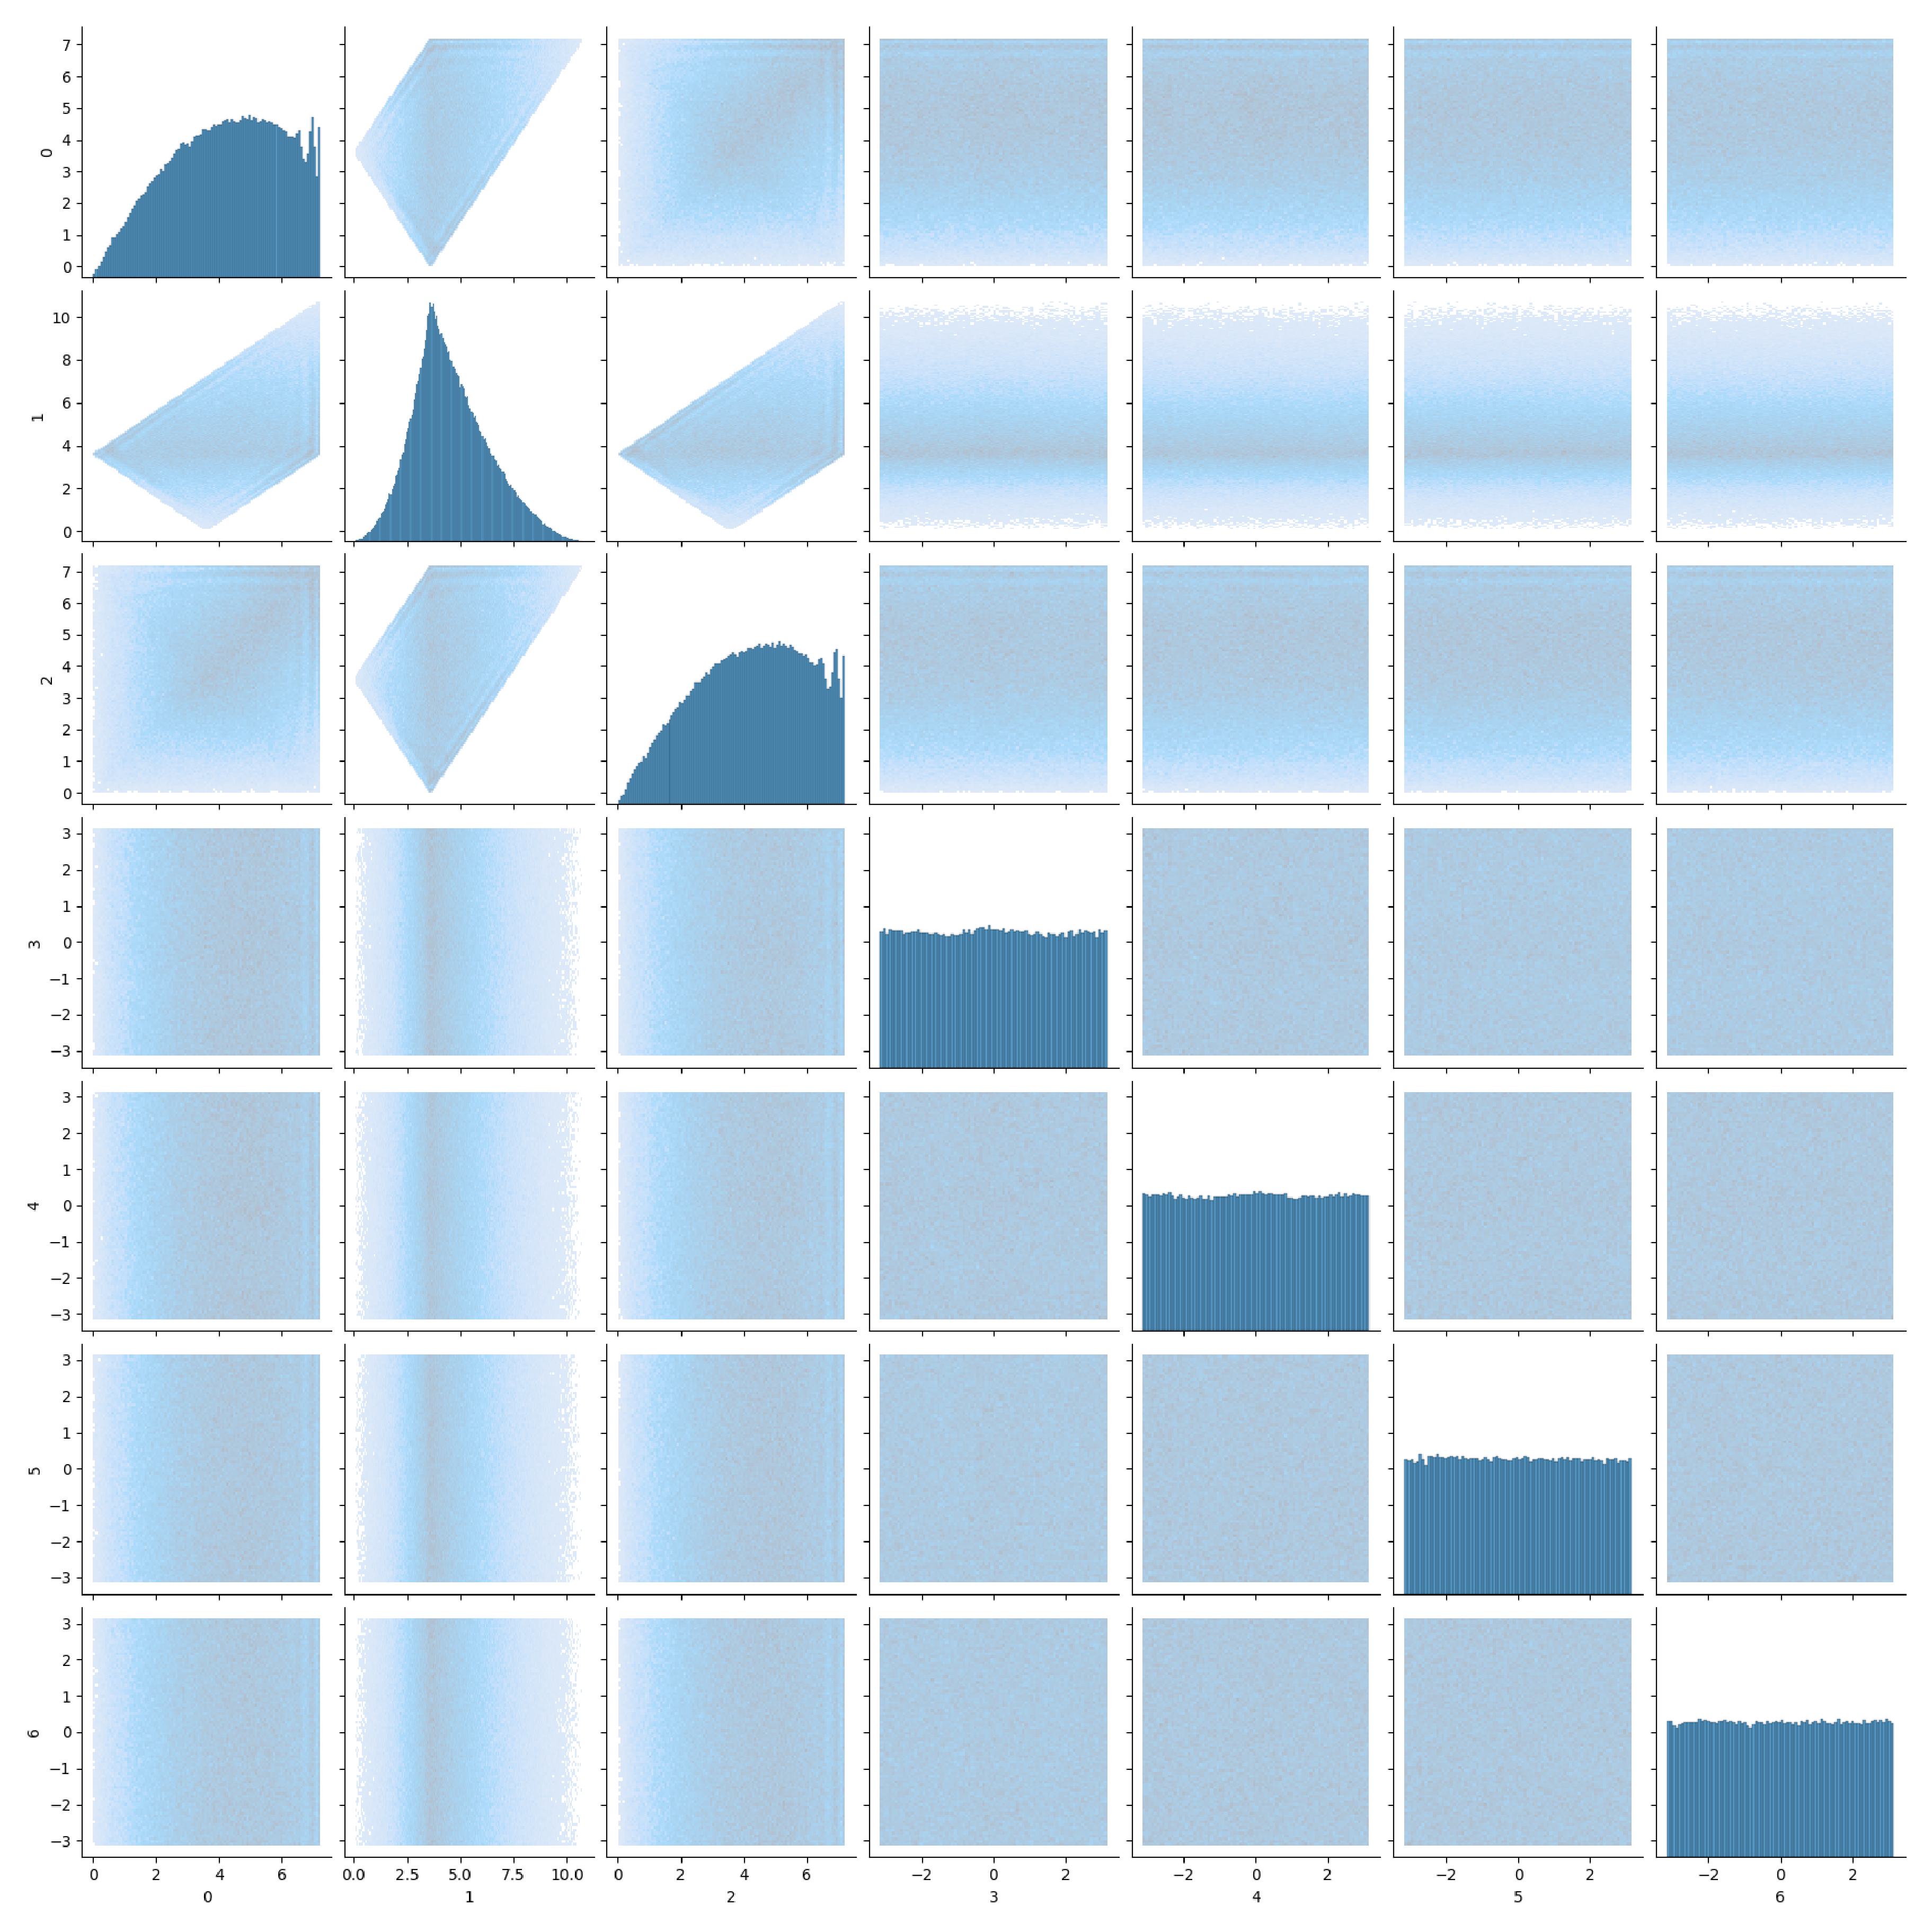
\includegraphics[width=0.4\textwidth]{images/constrained_diffusion/Positive Boundary, Backward Sampling, t=1.0.pdf}
	\caption{Reverse process samples for the cyclic peptide dataset from~\Cref{subsec:protein_loops} at \(t=1.0,0.9\) (left and right respectively) trained without the scaling function.}
	\label{fig:no_scaling}
\end{figure}

\begin{figure}[H]
	\centering
	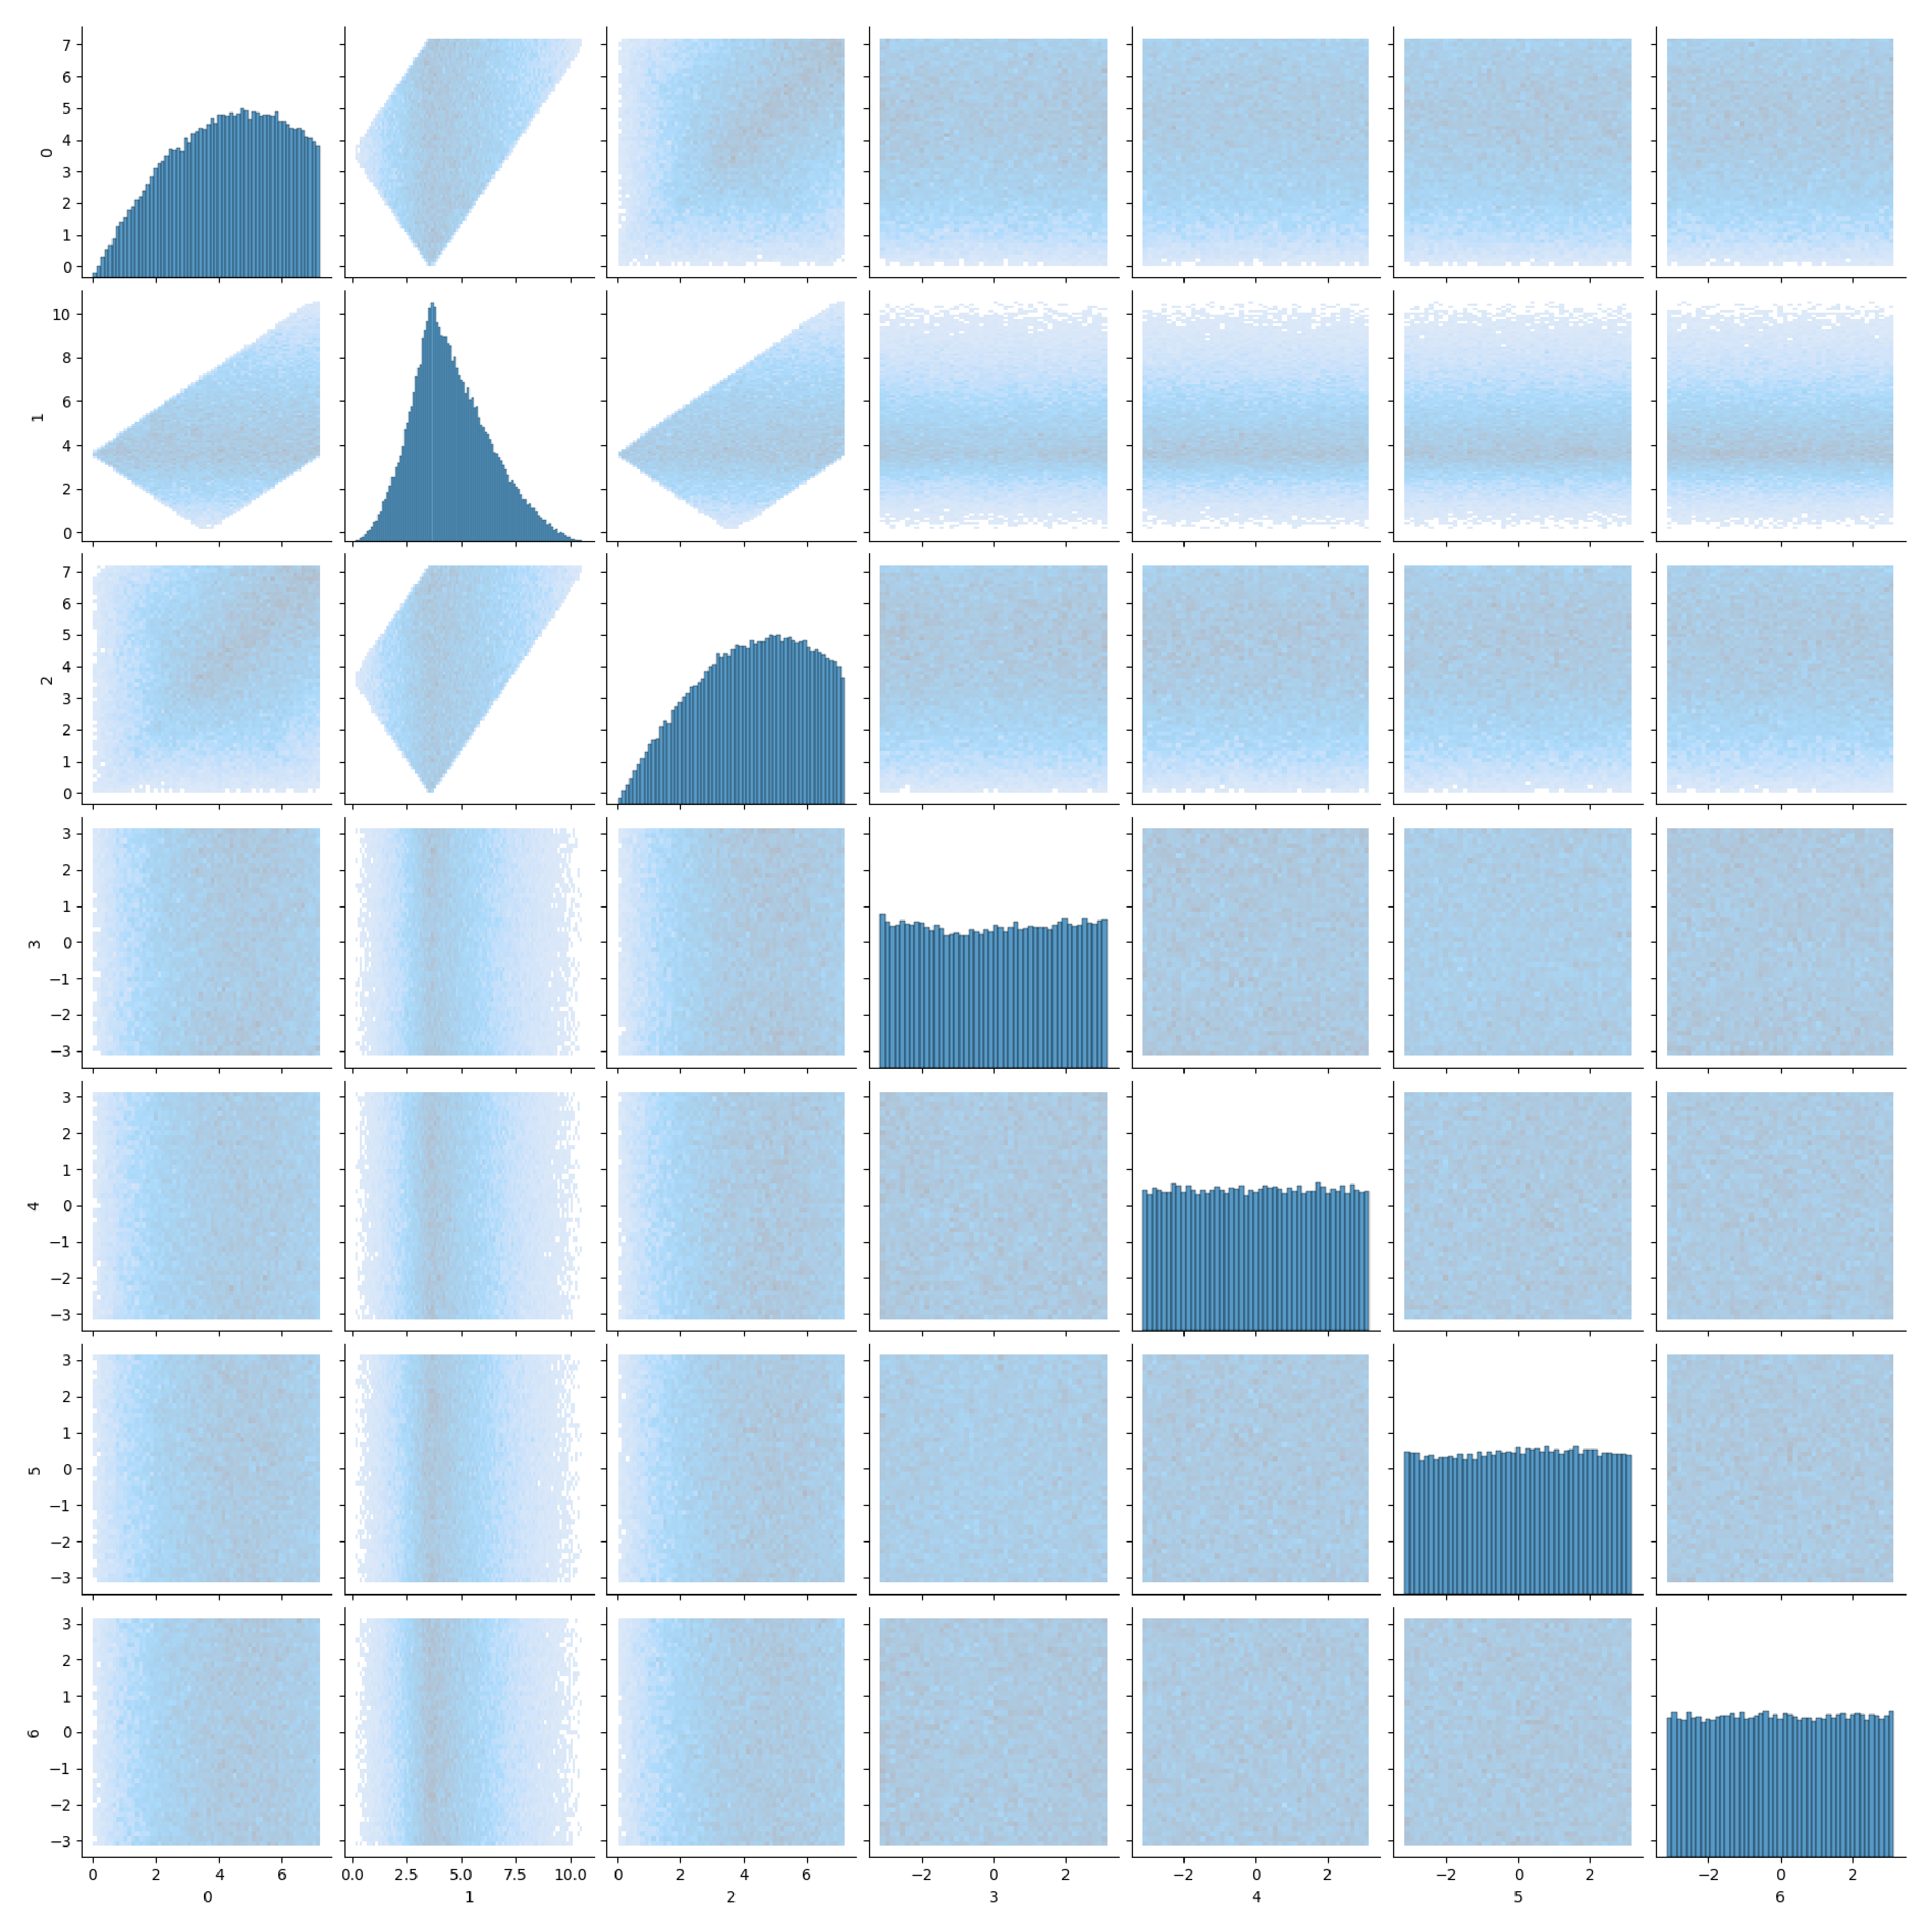
\includegraphics[width=0.4\textwidth]{images/constrained_diffusion/Zero Boundary, Backward Sampling, t=0.9.pdf}
	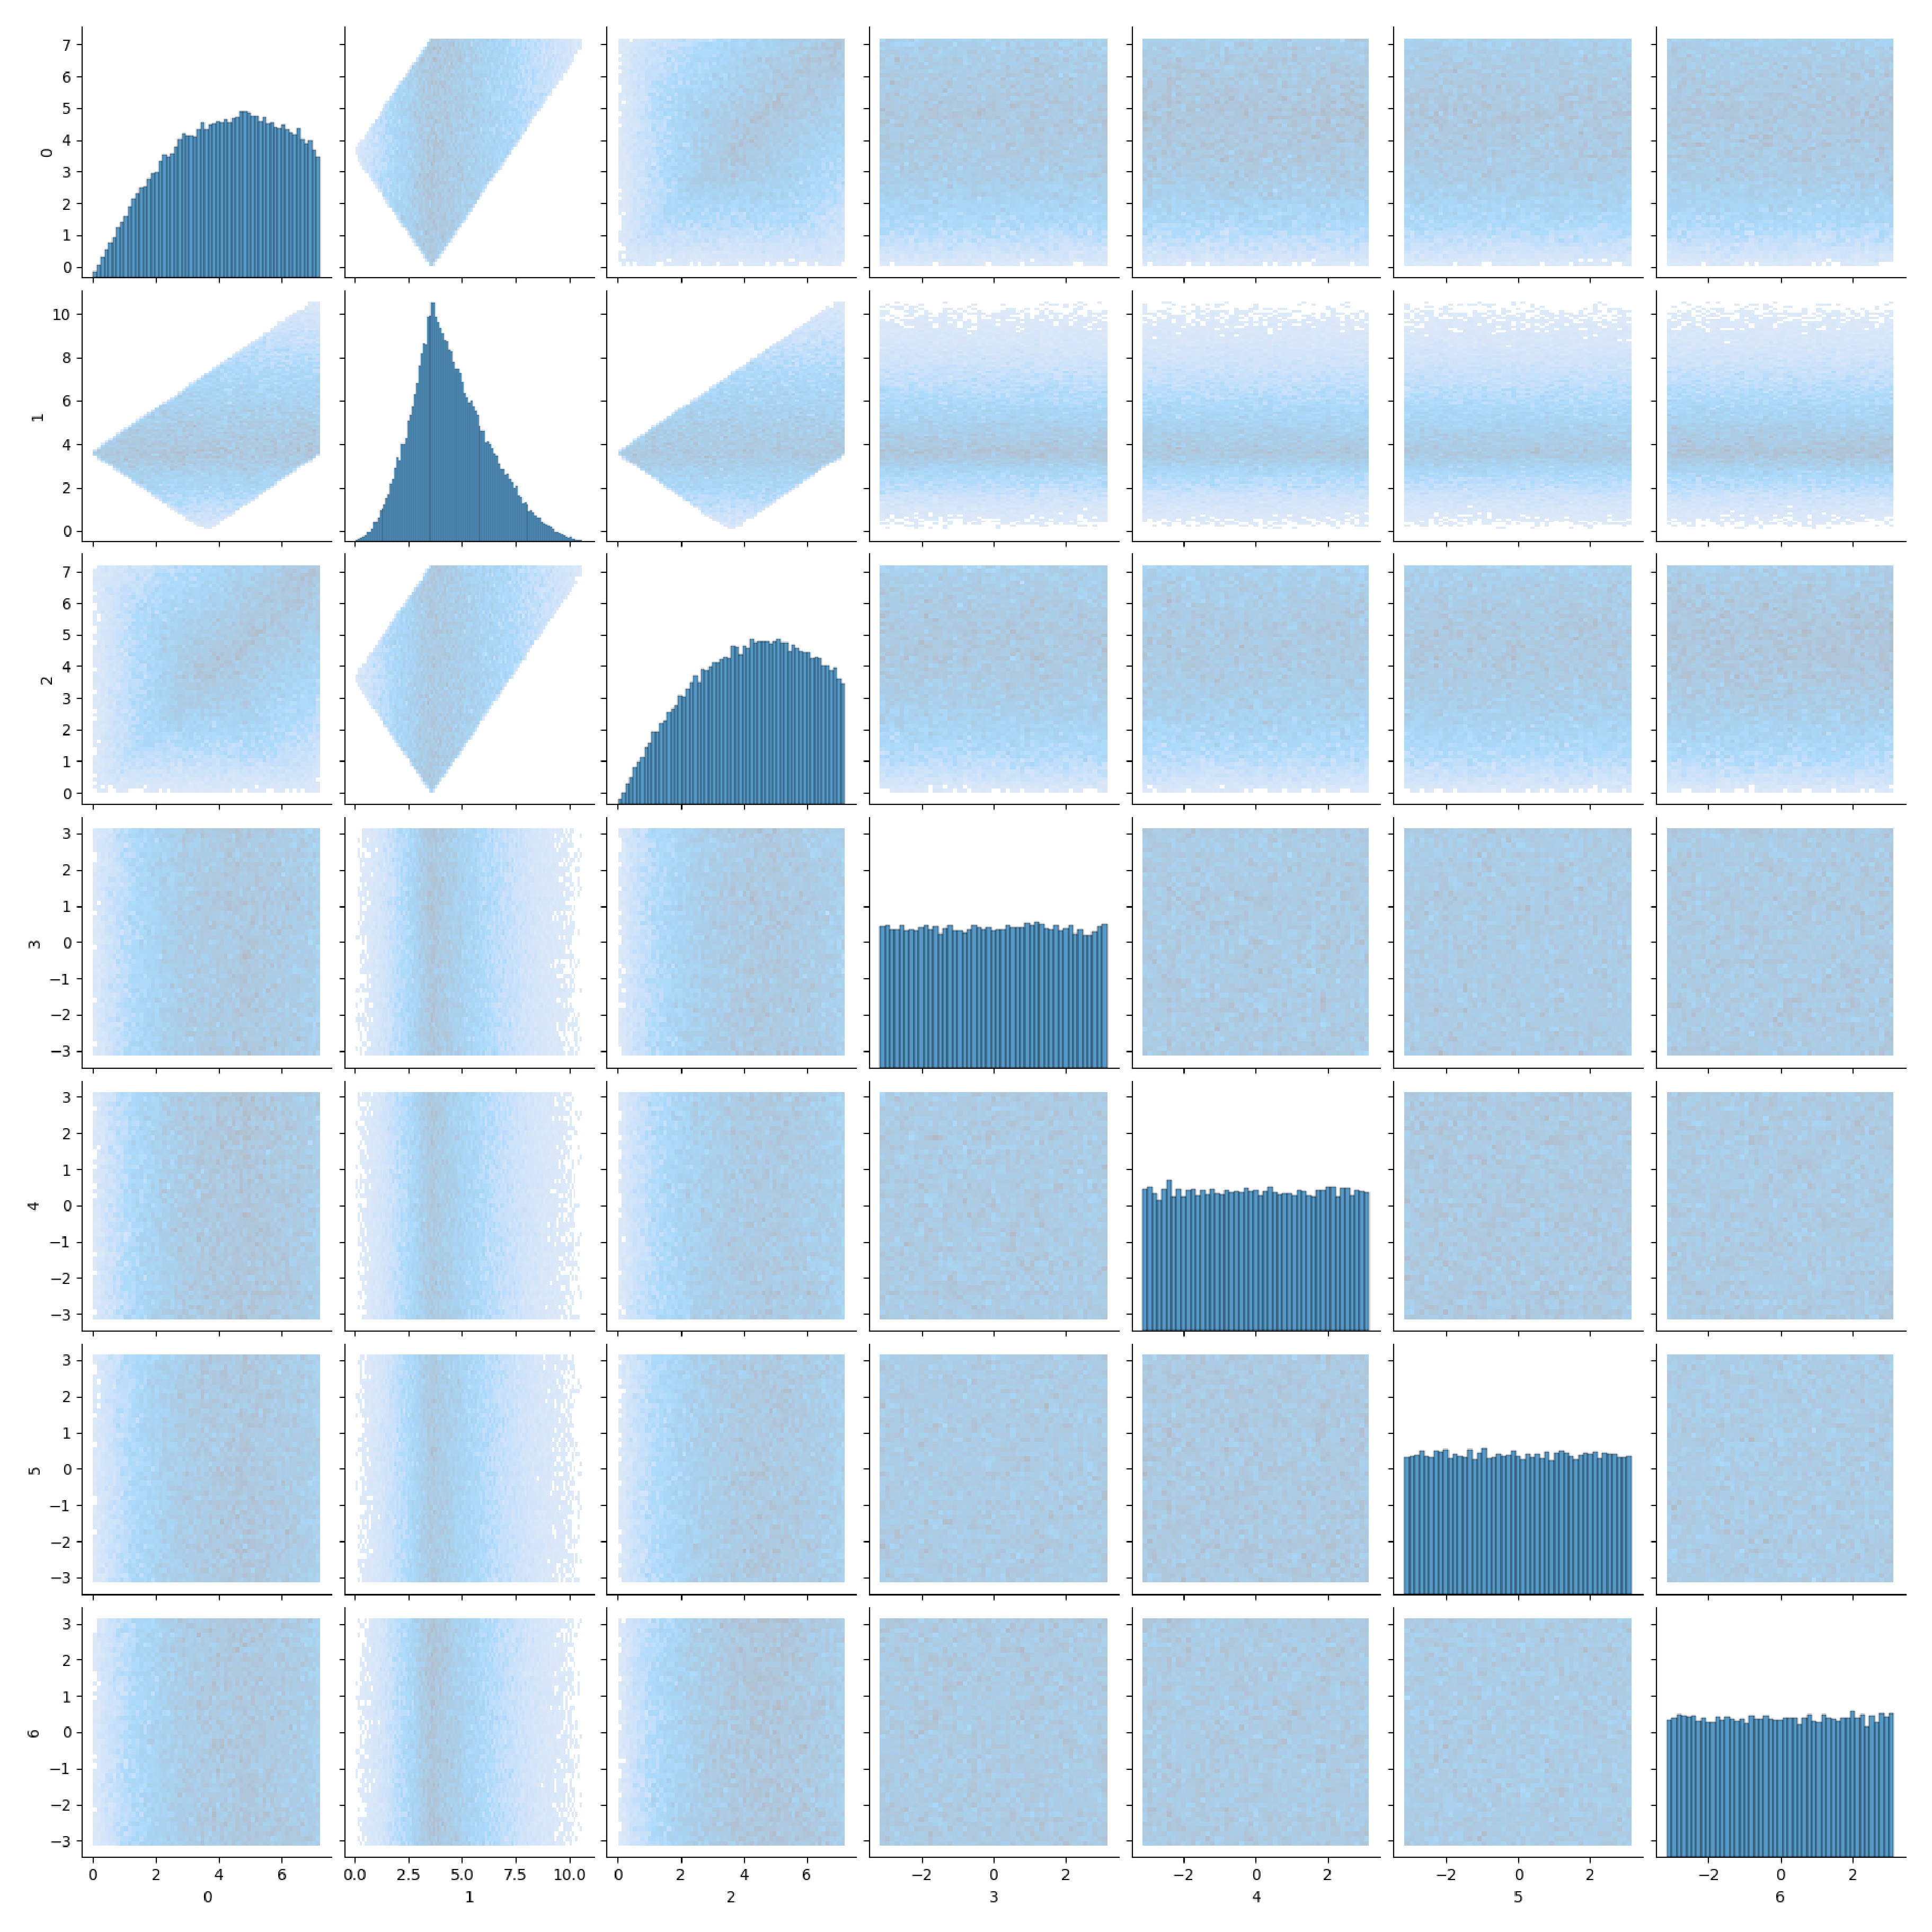
\includegraphics[width=0.4\textwidth]{images/constrained_diffusion/Zero Boundary, Backward Sampling, t=1.0.pdf}
	\caption{Reverse process samples for the cyclic peptide dataset from~\Cref{subsec:protein_loops} at \(t=1.0,0.9\) (left and right respectively) trained with the scaling function.}
	\label{fig:scaling}
\end{figure}

\section{Proof of \cref{thm:reflected_likelihood_ode}}
\label{sec:likel-eval}

\begin{proof}
	Since the distributions of \((\bar{\mathbf{B}}_t)_{t \in \cbr{0,T}}\) and \((\mathbf{X}_t)_{t \in \cbr{0,T}}\) satisfy the same Fokker-Planck equation whenever these processes are well-defined.
	Therefore, we first show that the process \((\mathbf{X}_t)_{t \in \cbr{0,T}}\) is well-defined and stay in \(\mathcal{M}\) at all times.
	Using \cite[Theorem 2.2]{burdzy2004heat}, we have that \(\partial p_t(x) = \tfrac{1}{2} \mathrm{div}(\nabla \log p_t)(x)\), for any \(t > 0\) and \(x \in \c{M}\).
	Next, we define \(\mathrm{d} \v{X}_t = \tfrac{1}{2} \nabla \log p_t(\v{X}_t) \mathrm{d} t\).
	Note that \((\v{X}_t)_{t \geq 0}\) is defined up to an explosion time \(T_\infty\) after which we fix \(\v{X}_t = \infty\).
	Denote \(T_0\) the first time such that \(\v{X}_t \in \partial \c{M}\).
	Note that since \(p_0\) is supported on \(\c{M}\) we have \(T_0 > 0\).
	We denote \((\v{Y}_t)_{t \in \cbr{0,T_0}} = (\v{X}_{T_0-t})_{t \in \cbr{0,T_0}}\).
	We have that for any \(t \in \cbr{0,T_0}\), \(\mathrm{d} \v{Y}_t = -\tfrac{1}{2} \nabla \log p_{T_0-t}(\v{Y}_t) \mathrm{d} t\).
	Since \((t,x) \mapsto \nabla \log p_t(x)\) is smooth on \(\cobr{0,+\infty} \times \partial \c{M}\), we get that for any \(t \in \cbr{0,T_0}\), \(\v{Y}_t \in \partial \c{M}\).
	In particular, we have that \(\v{Y}_{T_0/2} = \v{X}_{T_0/2} \in \partial \c{M}\) which is absurd.
	Therefore \(T_0 = +\infty\) (which also implies that \(T_\infty = +\infty\)).
	Hence, \((\v{X}_t)_{t \geq 0}\) is a flow on \(\c{M}\) and therefore for any \(t \geq 0\), the density \(q_t\) of \(\v{X}_t\) is smooth and satisfies \(\partial_t q_t(x) = -\tfrac{1}{2} \mathrm{div}(q_t \nabla \log p_t )(x)\).
	We conclude using the uniqueness of the solutions to the transport equation for smooth initialisation and coefficients on \(\R^d\).
\end{proof}

\section{Time-reversal for reflected Brownian motion}
\label{sec:time-revers-refl}

We start with the following definition.

\begin{definition}
	Let \(\c{M} \subset \R^d\) be an open set.
	\(\c{M}\) has a smooth boundary if for any
	\(x \in \partial \c{M}\), there exists \(\mathsf{U} \subset \R^d\) open and
	\(f \in \mathrm{C}^\infty(\mathsf{U}, \R)\) such that \(x \in \mathsf{U}\) and
	\begin{enumerate*}[label=(\alph*)]
		\item \(\mathrm{cl}(\c{M}) \cap \mathsf{U} = \cbr{x \in \mathsf{U} \; : \; f(x) \leq 0}\),
		\item \(\nabla f(x) \neq 0\) for any \(x \in \mathsf{U}\)
	\end{enumerate*}
	where \(\mathrm{cl}(\c{M})\) is the closure of \(\c{M}\).
\end{definition}

We will make the use of the following lemma which is a straightforward extension of \textcite[Theorem 2.6]{burdzy2004heat}.
The surface measure is defined in \cite[Proposition 2.43]{lee2006riemannian}.
Under mild regularity assumptions, it corresponds to the Hausdorff measure of \(\partial \c{M}\), see \cite{evans2015measure}.

\begin{lemma}
	\label{lemma:formula_integration}
	Let \(u\) such that \(s \mapsto u(s,x) \in \mathrm{C}^1(\del{0,T}, \R)\), for any \(s \in \del{0,T}\), \(x \mapsto u(s,x) \in \mathrm{C}^2(\mathrm{\c{M}}, \R)\) and \(u \in \mathrm{C}^1(\mathrm{cl}(\mathrm{\c{M}}), \R)\).
	Then for any \(T \geq 0\), \(s, t \in \cbr{0,T}\), we have \begin{equation} {\E\sbr{\int_s^t u(w, \bar{\v{B}}_w) \mathrm{d} \v{k}_w } = \tfrac{1}{2} \int_s^t \int_{\partial \c{M}} u(x) p_w(x) \mathrm{d} \sigma(x) \mathrm{d} w .
		}
	\end{equation}
\end{lemma}

Note that we recover \textcite[Theorem 2.6]{burdzy2004heat} if we set \(u=1\).
We also emphasize that the result of \textcite[Theorem 2.6]{burdzy2004heat} is stronger than \Cref{lemma:formula_integration} as it holds not only in expectation but also in \(\mathrm{L}^2\) and almost surely.

We are now ready to prove \Cref{sec:time-reversal-reflected}.
We follow the approach of \cite{petit1997Time} which itself is based on an extension of \cite{haussmann1986time}.
We refer to \textcite{cattiaux2021time} for recent entropic approaches of time-reversal.
Recall that \((\bar{\v{B}}_t, \v{k}_t)_{t \geq 0}\) is a solution to the \emph{Skorokhod problem} \parencite{skorokhod1961stochastic} if \((\v{k}_t)_{t \geq 0}\) a bounded variation process and \((\bar{\v{B}}_t)_{t \geq 0}\) a continuous adapted process such that for any \(t \geq 0\), \(\v{B}_t = \bar{\v{B}}_t + \v{k}_t \in \c{M}\), \((\bar{\v{B}}_t)_{t \geq 0}\) and \begin{equation} \label{eq:skorokhod_app} {\abs{\v{k}}_t = \int_0^t \mathbf{1}_{\bar{\v{B}}_s \in \partial \c{M}} \mathrm{d} \abs{\v{k}}_s , \quad \v{k}_t = \int_0^t \v{n}(\bar{\v{B}}_s) \mathrm{d} \abs{\v{k}}_s ,} \end{equation} In what follows, we define \((\v{Y}_t)_{t \in \cbr{0,T}}\) such that for any \(t \in \cbr{0,T}\), \(\v{Y}_t = \bar{\v{B}}_{T-t}\).
Let us consider the process \((\tilde{\v{B}}_t)_{t \in \cbr{0,T}}\) defined for any \(t \in \cbr{0,T}\) by \begin{equation} {\tilde{\v{B}}_t = -\bar{\v{B}}_T + \bar{\v{B}}_{T-t} + \v{k}_T - \v{k}_{T-t} - \int_{T-t}^T \nabla \log p_s(\bar{\v{B}}_s) \mathrm{d} s .
	}
\end{equation}
First, note that \(t \mapsto \tilde{\v{B}}_t\) is continuous.
Denote by \(\mathcal{F}\), the filtration associated with \((\bar{\v{B}}_{T-t})_{t \in \cbr{0,T}}\).
We have that \((\tilde{\v{B}}_t)_{t \in \cbr{0,T}}\) is adapted to \((\bar{\v{B}}_{T-t})_{t \in \cbr{0,T}}\).
Even more so, we have that \((\tilde{\v{B}}_t)_{t \in \cbr{0,T}}\) satisfies the strong Markov property since \((\bar{\v{B}}_t)_{t \in \cbr{0,T}}\) also satisfies the strong Markov property.
Let \(g \in \mathrm{C}_c^\infty(\mathrm{cl}(\c{M}))\) and consider for any \(0 \leq s \leq t \leq T\), \(\E\sbr{(\tilde{\v{B}}_t - \tilde{\v{B}}_s)g(\bar{\v{B}}_{T-t})}\).
For any \(0 \leq s \leq t \leq T\) we have \begin{equation} \label{eq:first_equality} \E\sbr{(\tilde{\v{B}}_t - \tilde{\v{B}}_s)g(\bar{\v{B}}_{T-t})} = {\E\sbr{(-\bar{\v{B}}_{T-s} + \bar{\v{B}}_{T-t} + \v{k}_{T-s} - \v{k}_{T-t} - \int_{T-t}^{T-s} \nabla \log p_u(\bar{\v{B}}_u) \mathrm{d} u) g(\bar{\v{B}}_{T-t})} .
	}
\end{equation}
In what follows, we prove that for any \(0 \leq s \leq t \leq T\) we have \(\E\sbr{(\tilde{\v{B}}_t - \tilde{\v{B}}_s)g(\bar{\v{B}}_{T-t})} = 0\).
Therefore, we only need to prove that for any \(0 \leq s \leq t \leq T\) we have \begin{equation} \label{eq:second_equality} {\E\sbr{(-\bar{\v{B}}_{t} + \bar{\v{B}}_{s} + \v{k}_t - \v{k}_{s} - \int_{s}^{t} \nabla \log p_u(\bar{\v{B}}_u) \mathrm{d} u) g(\bar{\v{B}}_{t})}=0 .
	}
\end{equation}
Let \(t \in \ocbr{0,T}\).
We introduce \(u: \ \cbr{0,t} \times \c{M}\) such that for any \(s \in \cbr{0,t}\) and \(x \in \c{M}\), \(u(s, x) = \E\sbr{g(\bar{\v{B}}_t) \vert \bar{\v{B}}_s=x}\).
Using \textcite[Theorem 2.8]{burdzy2004heat} we get that for any \(x \in \c{M}\), \(s \mapsto u(s,x) \in \mathrm{C}^1(\del{0,t}, \R)\) and for any \(s \in \del{0,t}\), \(x \mapsto u(s,x) \in \mathrm{C}^2(\mathrm{\c{M}}, \R)\) and \(x \mapsto u(s,x) \in \mathrm{C}^1(\mathrm{cl}(\c{M}), \R)\).
In addition, we have that for any \(s \in \del{0,t}\) and for any \(x \in \c{M}\) and \(x_0 \in \partial \c{M}\) \begin{equation} \label{eq:backward_kolmogorov_dupref} {\partial_s u(s,x) + \tfrac{1}{2} \Delta u(s,x) = 0 , \qquad \langle \nabla u(s, x_0), \v{n}(x_0) \rangle = 0 .
	}
\end{equation}
This equation is called the backward Kolmogorov equation.
Using \eqref{eq:backward_kolmogorov_dupref}, \(\bar{\v{B}}_t = \v{B}_t - \v{k}_t\) for any \(t \geq 0\) and the It\^o formula for semimartingale \parencite[Chapter IV, Theorem 3.3]{revuz2013continuous} we have that for any \(s \in \del{0,t}\) \begin{align} \E\sbr{u(t, \bar{\v{B}}_t)\bar{\v{B}}_t} & {= \E\sbr{u(s, \bar{\v{B}}_s)\bar{\v{B}}_s} + \E\sbr{\tfrac{1}{2} \int_s^t \bar{\v{B}}_w \Delta u(w, \bar{\v{B}}_w) \mathrm{d} w}} {+\E\sbr{\int_s^t \nabla u(w, \bar{\v{B}}_w) \mathrm{d} w }} \\ & \qquad {- \E\sbr{\int_s^t \bar{\v{B}}_w \langle \nabla u(w, \bar{\v{B}}_w), \v{n}(\bar{\v{B}}_w) \rangle \mathrm{d} \abs{\v{k}}_w}} \\ & \qquad {- \E\sbr{\int_s^t u(w,\bar{\v{B}}_w) \v{n}(\bar{\v{B}}_w) \mathrm{d} \abs{\v{k}}_w}} \\ & \qquad {+ \E\sbr{\int_s^t \bar{\v{B}}_w \partial_w u(w, \bar{\v{B}}_w) \mathrm{d} w} } \\ & {= \E\sbr{u(s, \bar{\v{B}}_s)\bar{\v{B}}_s} {+\E\sbr{\int_s^t \nabla u(w, \bar{\v{B}}_w) \mathrm{d} w }}} {- \E\sbr{\int_s^t u(w,\bar{\v{B}}_w) \v{n}(\bar{\v{B}}_w) \mathrm{d} \abs{\v{k}}_w}} \label{eq:intermediate} \end{align} In addition, using the Fubini theorem and the definition of \(\v{k}_t\) we have that for any \(s \in \del{0,t}\) \begin{equation} {\E\sbr{\int_s^t u(w,\bar{\v{B}}_w) \v{n}(\bar{\v{B}}_w) \mathrm{d} \abs{\v{k}}_w} = \E\sbr{\int_s^t \E\sbr{g(\bar{\v{B}}_t) \vert \bar{\v{B}}_w} \v{n}(\bar{\v{B}}_w) \mathrm{d} \abs{\v{k}}_w} = \E\sbr{g(\bar{\v{B}}_t)(\v{k}_t - \v{k}_s)} .
	} \label{eq:boundary_uno}
\end{equation}
Finally, using the divergence theorem and \textcite[Theorem 2.6]{burdzy2004heat} we have that for any \(s \in \del{0,t}\) \begin{align} {\E\sbr{\int_s^t \nabla u(w, \bar{\v{B}}_w) \mathrm{d} w }} & = {\int_s^t \int_\c{M} \nabla u(w, x) p_w(x) \mathrm{d} x \mathrm{d} w } \\ & = - {\int_s^t \int_\c{M} u(w, x) \nabla \log (p_w(x)) p_w(x) \mathrm{d} x \mathrm{d} w + \int_s^t \int_{\partial \c{M}} u(w,x) p_w(x) \mathrm{d} x \mathrm{d} \sigma(w)} , \end{align} where \(\sigma\) is the surface area measure on \(\partial \c{M}\), see \textcite{burdzy2004heat}.
Using \Cref{lemma:formula_integration} and the Fubini theorem we get that \begin{align} {\E\sbr{\int_s^t \nabla u(w, \bar{\v{B}}_w) \mathrm{d} w }} & = - {\int_s^t \int_\c{M} u(w, x) \nabla \log (p_w(x)) p_w(x) \mathrm{d} x \mathrm{d} w + \E\sbr{\int_s^t u(w, \bar{\v{B}}_w) \mathrm{d} \v{k}_w } } \\ & = - {\E\sbr{\int_s^t g(\bar{\v{B}}_t) \nabla \log (p_w(\bar{\v{B}}_w))\mathrm{d} w} + 2 \E\sbr{g(\bar{\v{B}}_t)(\v{k}_t - \v{k}_s) }} \label{eq:boundary_duo} \end{align} Combining \eqref{eq:intermediate}, \eqref{eq:boundary_uno} and \eqref{eq:boundary_duo} we get that \begin{equation} { \E\sbr{u(t, \bar{\v{B}}_t) } = \E\sbr{u(s, \bar{\v{B}}_s) } - \E\sbr{ g(\bar{\v{B}}_t)\int_s^t \nabla \log p_w(\bar{\v{B}}_w) \mathrm{d} w }} + { \E\sbr{g(\bar{\v{B}}_t)(\v{k}_t - \v{k}_s) }} .
\end{equation}
Therefore, we get \eqref{eq:second_equality} and \eqref{eq:first_equality}.
Hence, \((\tilde{\v{B}}_t)_{t \in \cbr{0,T}}\) is a continuous martingale.
In addition, we have that for any \(t \in \cbr{0,T}\), \(\E\sbr{\tilde{\v{B}}_t \tilde{\v{B}}_t^\top} = t \m{I}\) and therefore, \((\tilde{\v{B}}_t)_{t \in \cbr{0,T}}\) is a Brownian motion using the L\'evy characterisation of Brownian motion \parencite[Chapter IV, Theorem 3.6]{revuz2013continuous}.
Denote \((\v{j}_t)_{t \in \cbr{0,T}} = (\v{k}_T - \v{k}_{T-t})_{t \in \cbr{0,T}}\).
Using \eqref{eq:first_equality}, we have that for any \(t \in \cbr{0,T}\) \begin{equation} {\bar{\v{B}}_{T-t} = \bar{\v{Y}}_0 + \tilde{\v{B}}_t + \int_0^t \nabla \log p_{T-s}(\v{Y}_s) \mathrm{d} s - \v{j}_t .
	}
\end{equation}
Using \eqref{eq:skorokhod_app}, we have for any \(t \in \cbr{0,T}\) \begin{equation} {\abs{\v{j}}_t = \int_0^t \mathbf{1}_{\v{Y}_s \in \partial \c{M}} \mathrm{d} \abs{\v{j}}_s , \quad \v{j}_t = \int_0^t \v{n}(\bar{\v{Y}}_s) \mathrm{d} \abs{\v{j}}_s ,} \end{equation} which concludes the proof.
\section{Experimental details}
\label{sec:exp_details}

In what follows we describe the experimental settings used to generate results introduced in \cref{sec:experiments-constrained}.
~
The models and experiments have been implemented in Jax~\parencite{jax2018github}, using a modified version of the Riemannian geometry library Geomstats~\parencite{geomstats2020}.

\paragraph{Architecture.}
The architecture of the score network \(\bm{s}_\theta\) is given by a multilayer perceptron with \(6\) hidden layers with \(512\) units each.
We use sinusoidal activation functions.

\paragraph{Training.}
All models are trained by the stochastic optimizer Adam \parencite{kingma2014adam} with parameters \(\beta_1=0.9\), \(\beta_2=0.999\), batch-size of \(256\) data-points.
The learning rate is annealed with a linear ramp from \(0\) to \(1000\) steps, reaching the maximum value of \(2e-4\), and from then with a cosine schedule down to \(0\) after \(100k\) iterations in total.

\paragraph{Diffusion.}
Following \textcite{song2020score}, the diffusion models diffusion coefficient is parametrized as \(g(t) = \sqrt{\beta(t)}\) with \(\beta: \ t \mapsto \beta_{\min} + (\beta_{\max} - \beta_{\min}) \cdot t\), where we found \(\beta_{\min}=0.001\) and \(\beta_{\max}=6\) to work best.

\paragraph{Metrics.}
We measure the performance of trained models via the Maximum Mean Discrepancy (MMD) \parencite{gretton2012kernel}, which is a kernel based metric between two distributions \(P\) and \(Q\).
The MMD can be empirically approximated with the following U-statistics \(\mathrm{MMD}^2(P, Q) = \tfrac{1}{m(m-1)} \sum_i \sum_{j \neq i} k(x_i, x_j) + \tfrac{1}{m(m-1)} \sum_i \sum_{j \neq i} k(y_i, y_j) - 2 \tfrac{1}{m^2} \sum_i \sum_{j} k(x_i, y_j)\) with \(x_i \sim P\) and \(y_i \sim Q\), where \(k\) is a kernel.
For synthetic experiments we use a sum of weighted RBF kernels matching the generating distributions for the Gaussian mixtures.
For the other experiments we use an RBF kernel.
For all experiments we use 100,000 samples to compute the MMD.

\subsection{Synthetic data on polytopes}
\label{sec:app_synthetc_data}

\paragraph{Hypercube}

The hypercube is a specific instance of a convex polytope where the affine constraints are given by the following coefficients: 

\begin{equation} A = \begin{pmatrix} 1 & \dots & 0 \\ -1 & \dots & 0 \\ \vdots & \ddots & \vdots \\ 0 & \dots & 1 \\ 0 & \dots & -1 \\ \end{pmatrix}, \;\; b = \begin{pmatrix} 1 \\1\\\vdots\\1\\1 \end{pmatrix}.
\end{equation}

Where \(A\) is a \(2n \times n\) matrix and \(b\) an \(n\) dimensional vector.

We construct the training and test datasets by sampling for both \(100 000\) points from a mixture of `wrapped normal' distributions illustrated in \cref{fig:hypercube_data} and which density is given by \[ p_0(x) =& 0.7 ~\text{ReflectedStep}[(0.5,0.5), \cdot, \{f_i\}_{i \in \mathcal{I}}] \# \c{N}(0,0.25) \\&+ 0.3 ~\text{ReflectedStep}[(-0.5,-0.5), \cdot, \{f_i\}_{i \in \mathcal{I}}] \# \c{N}(0,0.25).
\]

\begin{figure}[H]
	\centering
	\begin{subfigure}{0.30\textwidth}
		\centering
		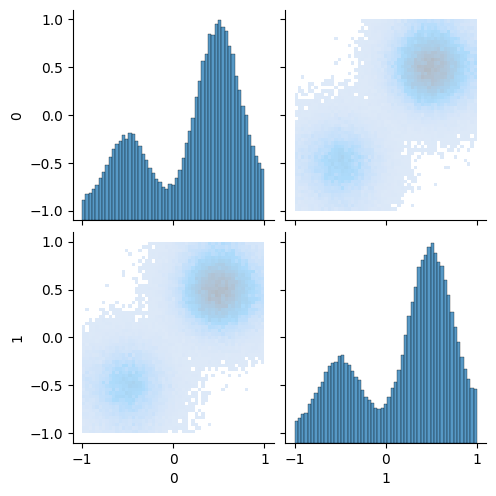
\includegraphics[width=\linewidth]{images/constrained_diffusion/hypercube_data.jpg}
		\caption{On the hypercube.}
		\label{fig:hypercube_data}
	\end{subfigure}
	\hspace{1.5cm}
	\begin{subfigure}{0.30\textwidth}
		\centering
		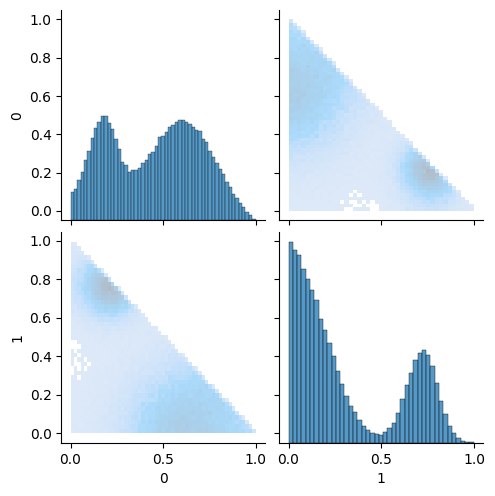
\includegraphics[width=\linewidth]{images/constrained_diffusion/simplex_data.jpg}
		\caption{On the simplex.}
		\label{fig:simplex_data}
	\end{subfigure}
	\caption{Pairwise and marginals samples from the synthetic data distribution.}
	\label{fig:synthetic_data}
\end{figure}

\paragraph{Simplex \(\Delta^n\).}

Similarly, to parametrise the simplex as a convex polytope we set the matrix and constraints to be given by 

\begin{equation} A = \begin{pmatrix} -1 & 0 & \dots & 0 \\ \vdots & \vdots & \ddots & \vdots \\ 0 & 0 & \dots & -1 \\ 1 & 1 & 1 & 1 \end{pmatrix}, \;\; b = \begin{pmatrix} 0 \\\vdots\\0\\1 \end{pmatrix}.
\end{equation}

Where \(A\) will be a \(n-1 \times n\) matrix.
Essentially we perform diffusion over the first \(n-1\) components of the simplex, allowing the last component to be determined by the one minus the sum of the first \(n-1\).

Similarly than for the hypercube, we construct the training and test datasets from generated data points which are illustrated in \cref{fig:simplex_data}.
The score network at different times is illustrated in \Cref{fig:simplex_score}.

\begin{figure}[H]
	\centering
	\begin{subfigure}{0.32\textwidth}
		\centering
		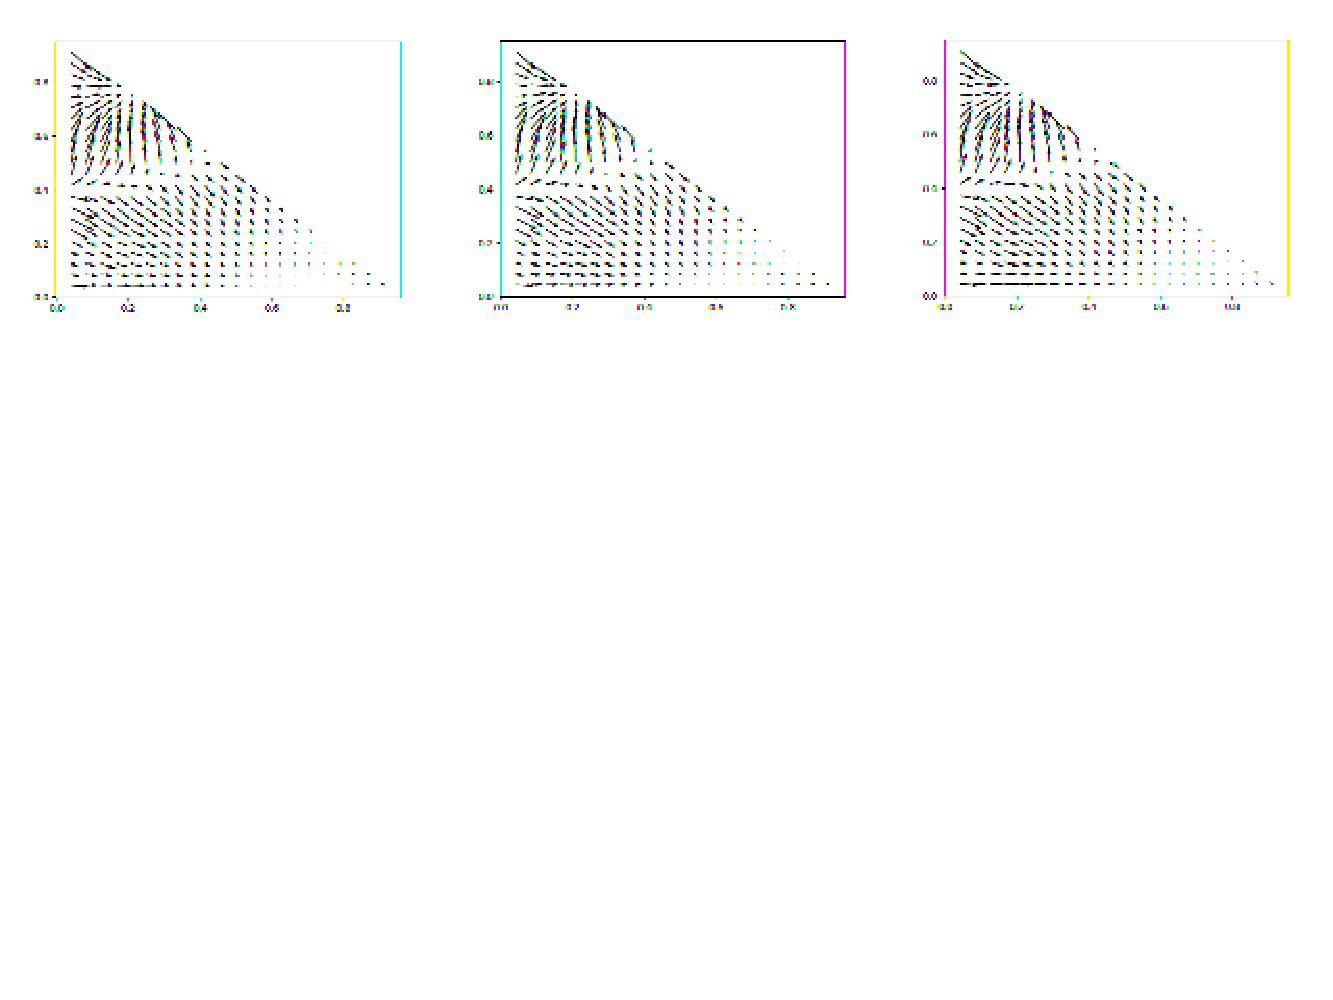
\includegraphics[width=\linewidth]{images/constrained_diffusion/score(1).pdf}
		\caption{\(t=0.01\).}
		\label{fig:001_score}
	\end{subfigure}
	\hfill
	\begin{subfigure}{0.32\textwidth}
		\centering
		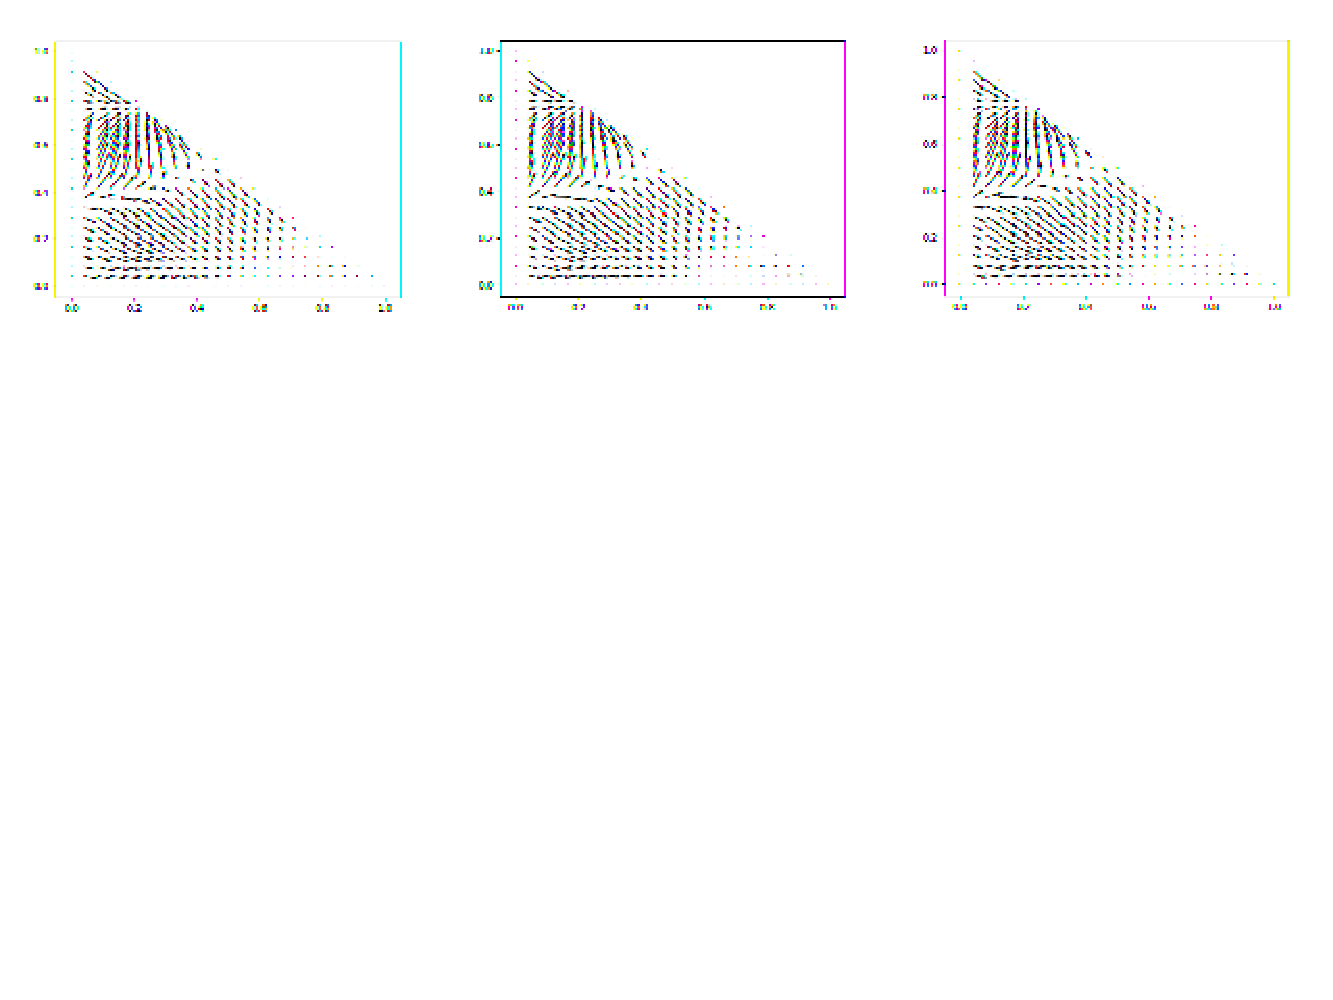
\includegraphics[width=\linewidth]{images/constrained_diffusion/score(2).pdf}
		\caption{\(t=0.5\).}
		\label{fig:05_score}
	\end{subfigure}
	\hfill
	\begin{subfigure}{0.26\textwidth}
		\centering
		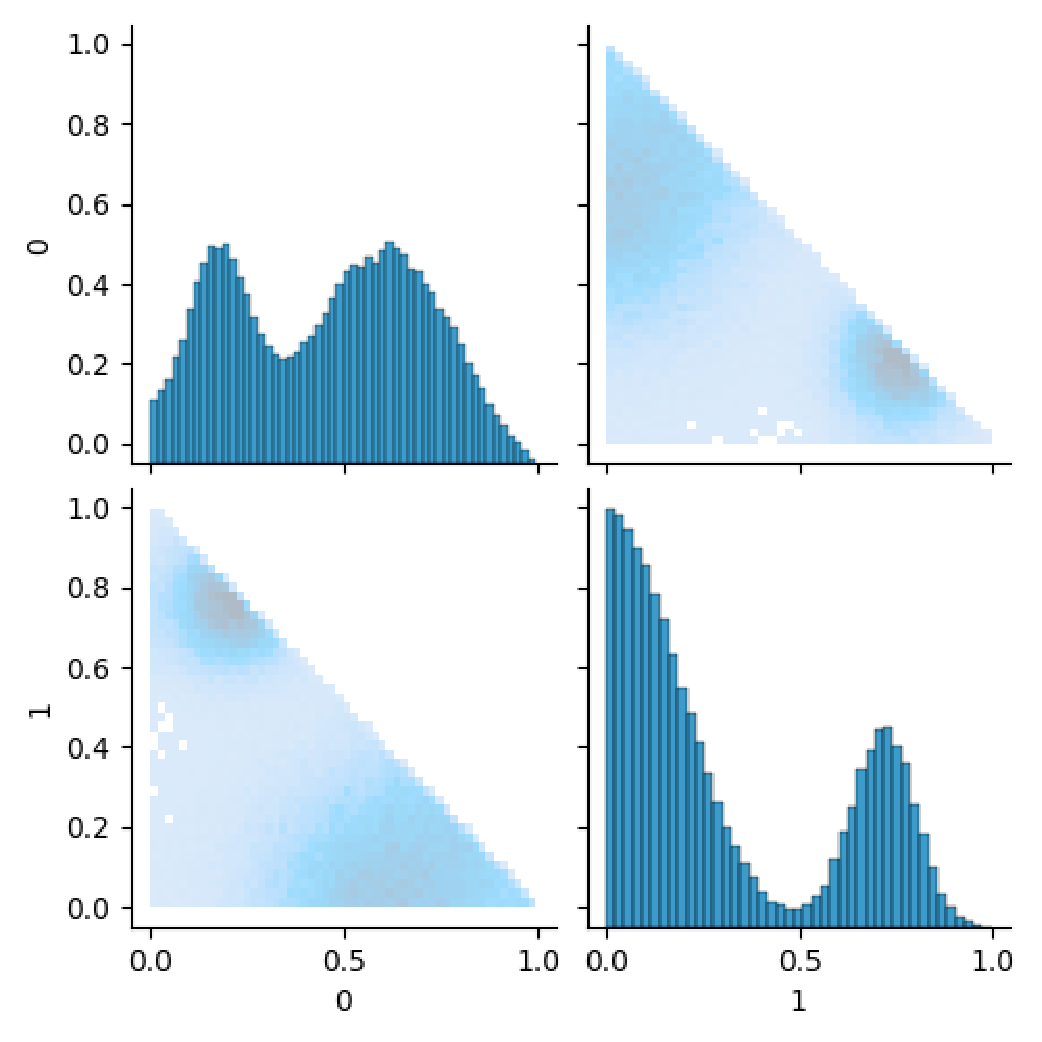
\includegraphics[width=\linewidth]{images/constrained_diffusion/score(4).pdf}
		\caption{Generated distribution.}
		\label{fig:generated}
	\end{subfigure}
	\caption{Evolution of the score on the simplex and generated distribution.}
	\label{fig:simplex_score}
\end{figure}

\paragraph{The Birkhoff polytope.}
The Birkhoff polytope is the space of doubly stochastic matrices, i.e.\ \(B_n = \{ \mathrm{P} \in [0,1]^{n \times n} : \sum_i^n P_{i,j}=1, \sum_j^n P_{i,j}=1\}\).
It is a convex polytope in \(\R^{n^2}\) and has dimension \(d = (n-1)^2\).

\begin{figure}[H]
	\centering
	\begin{subfigure}{0.3\textwidth}
		\centering
		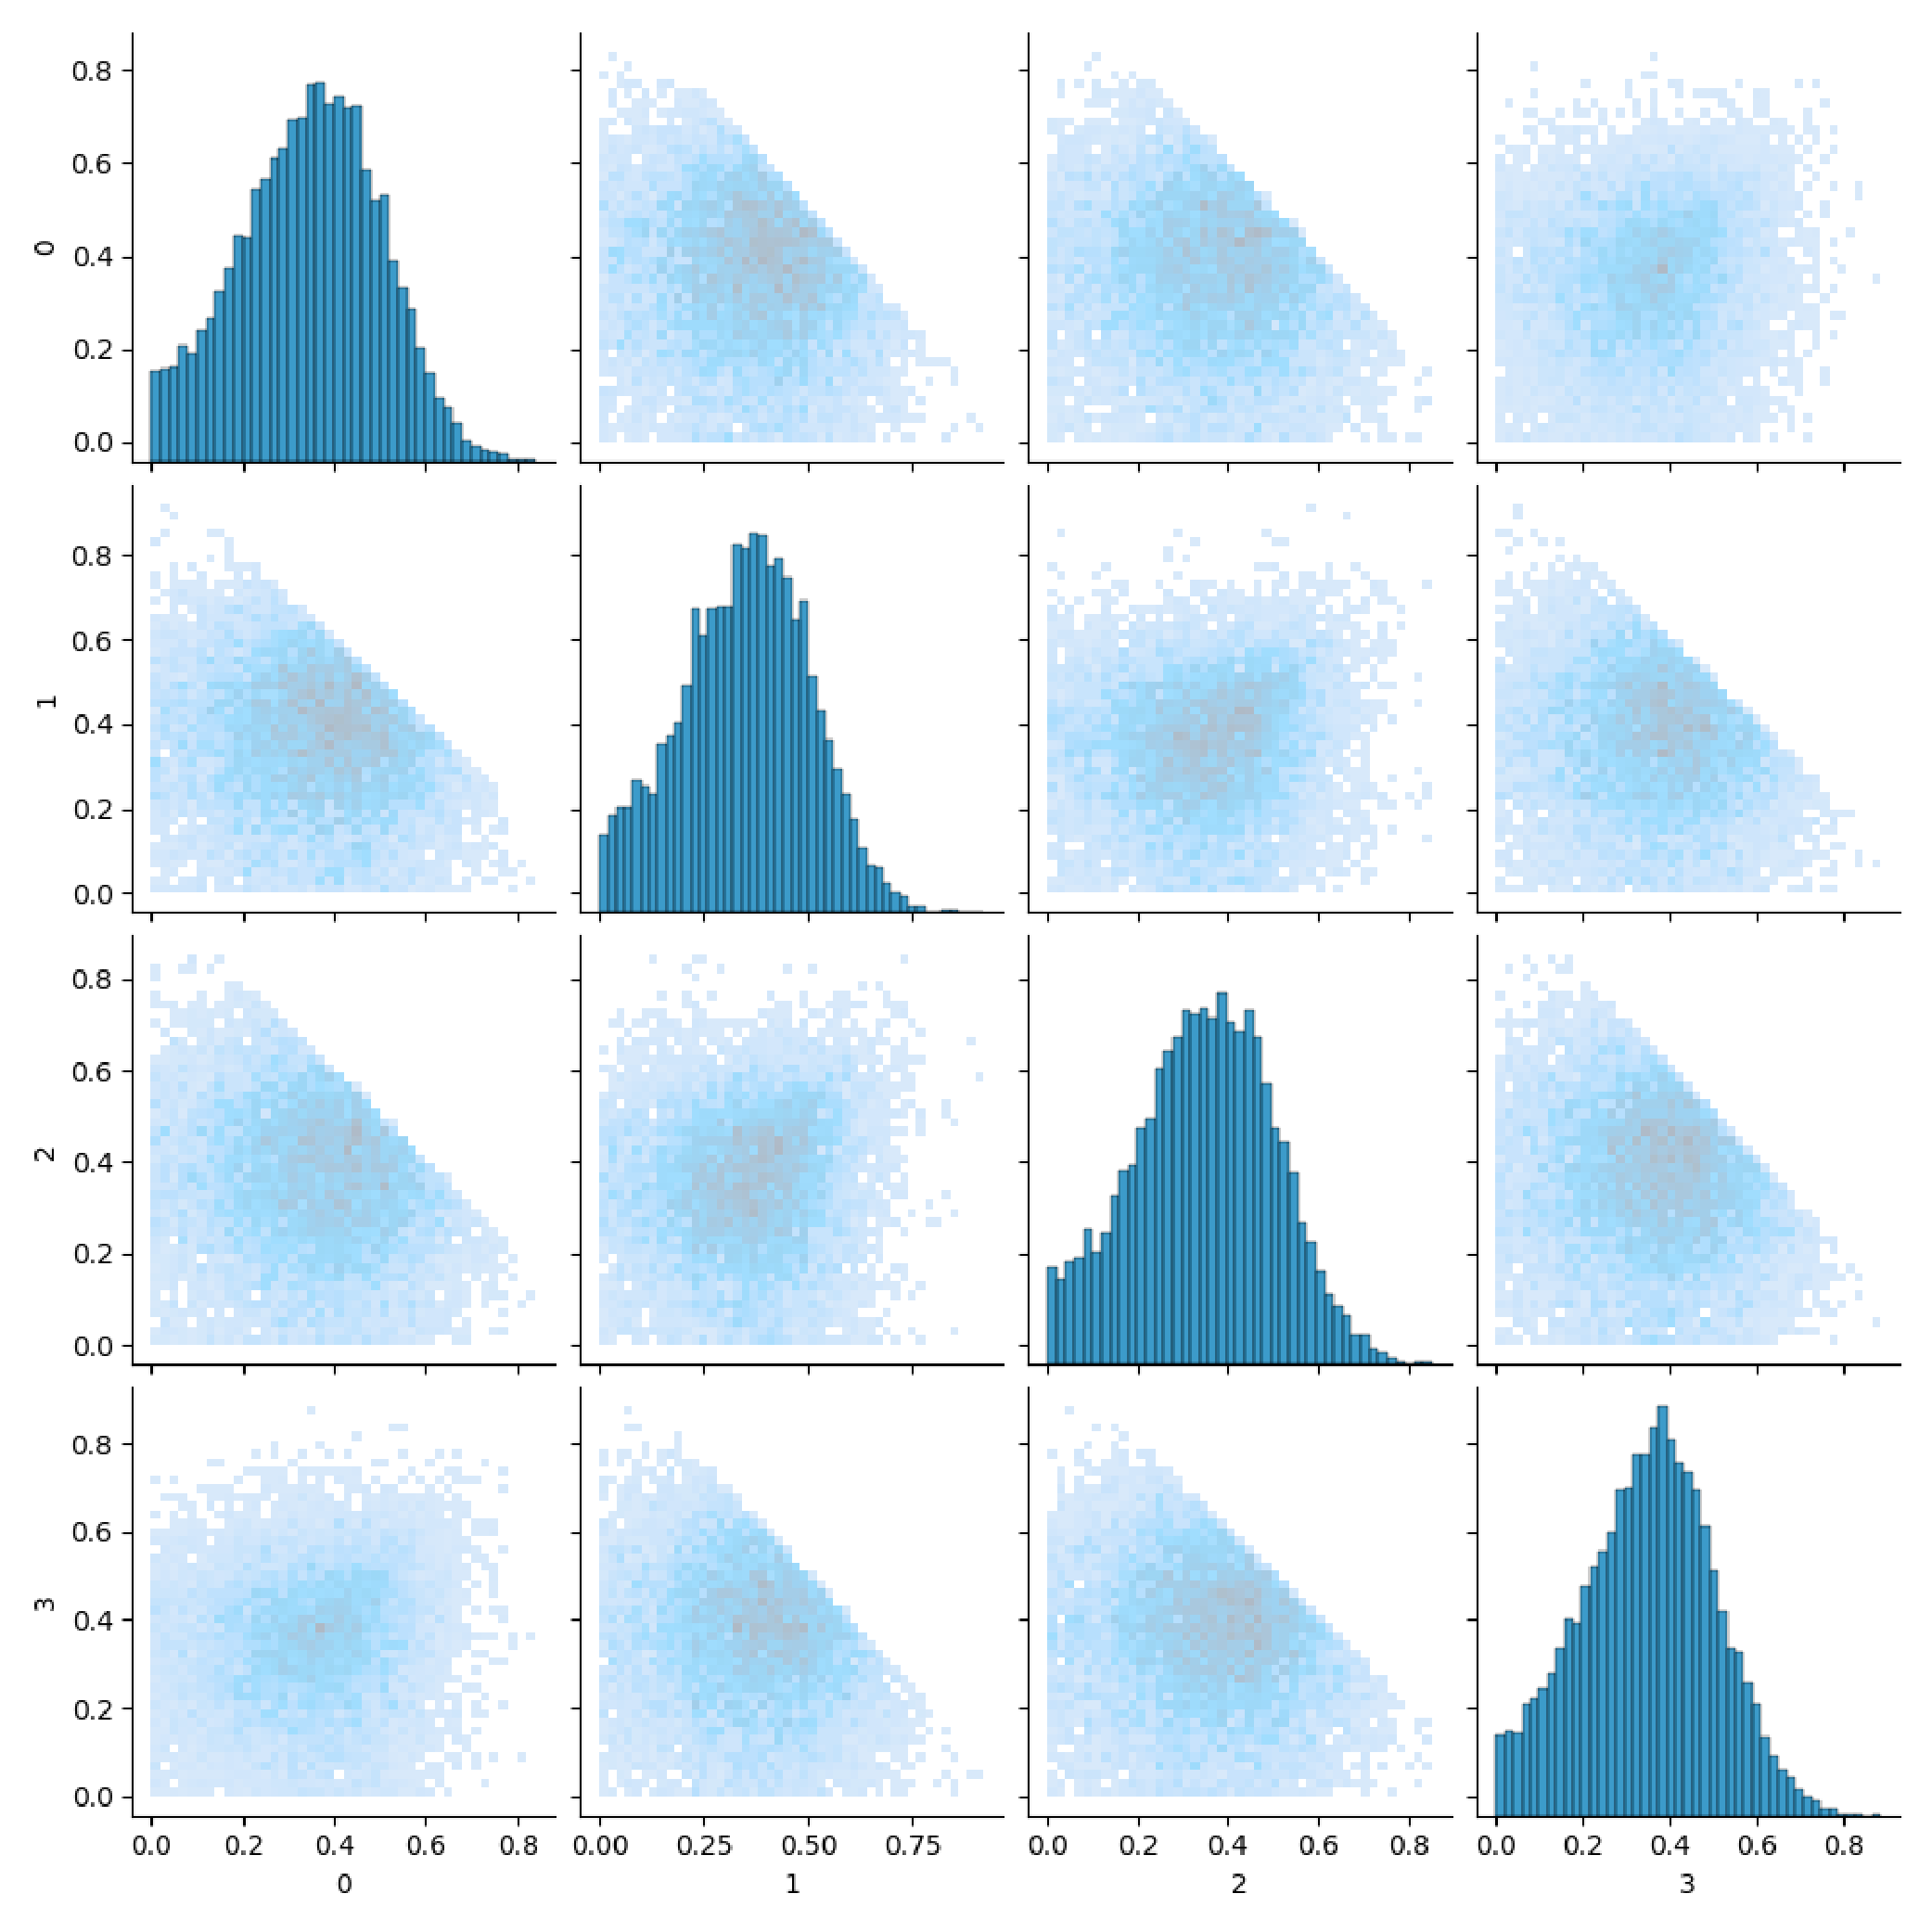
\includegraphics[width=\linewidth]{images/constrained_diffusion/birkhoff_data.pdf}
		\caption{Data.}
		\label{fig:birkhoff_data}
	\end{subfigure}
	\hfill
	\begin{subfigure}{0.3\textwidth}
		\centering
		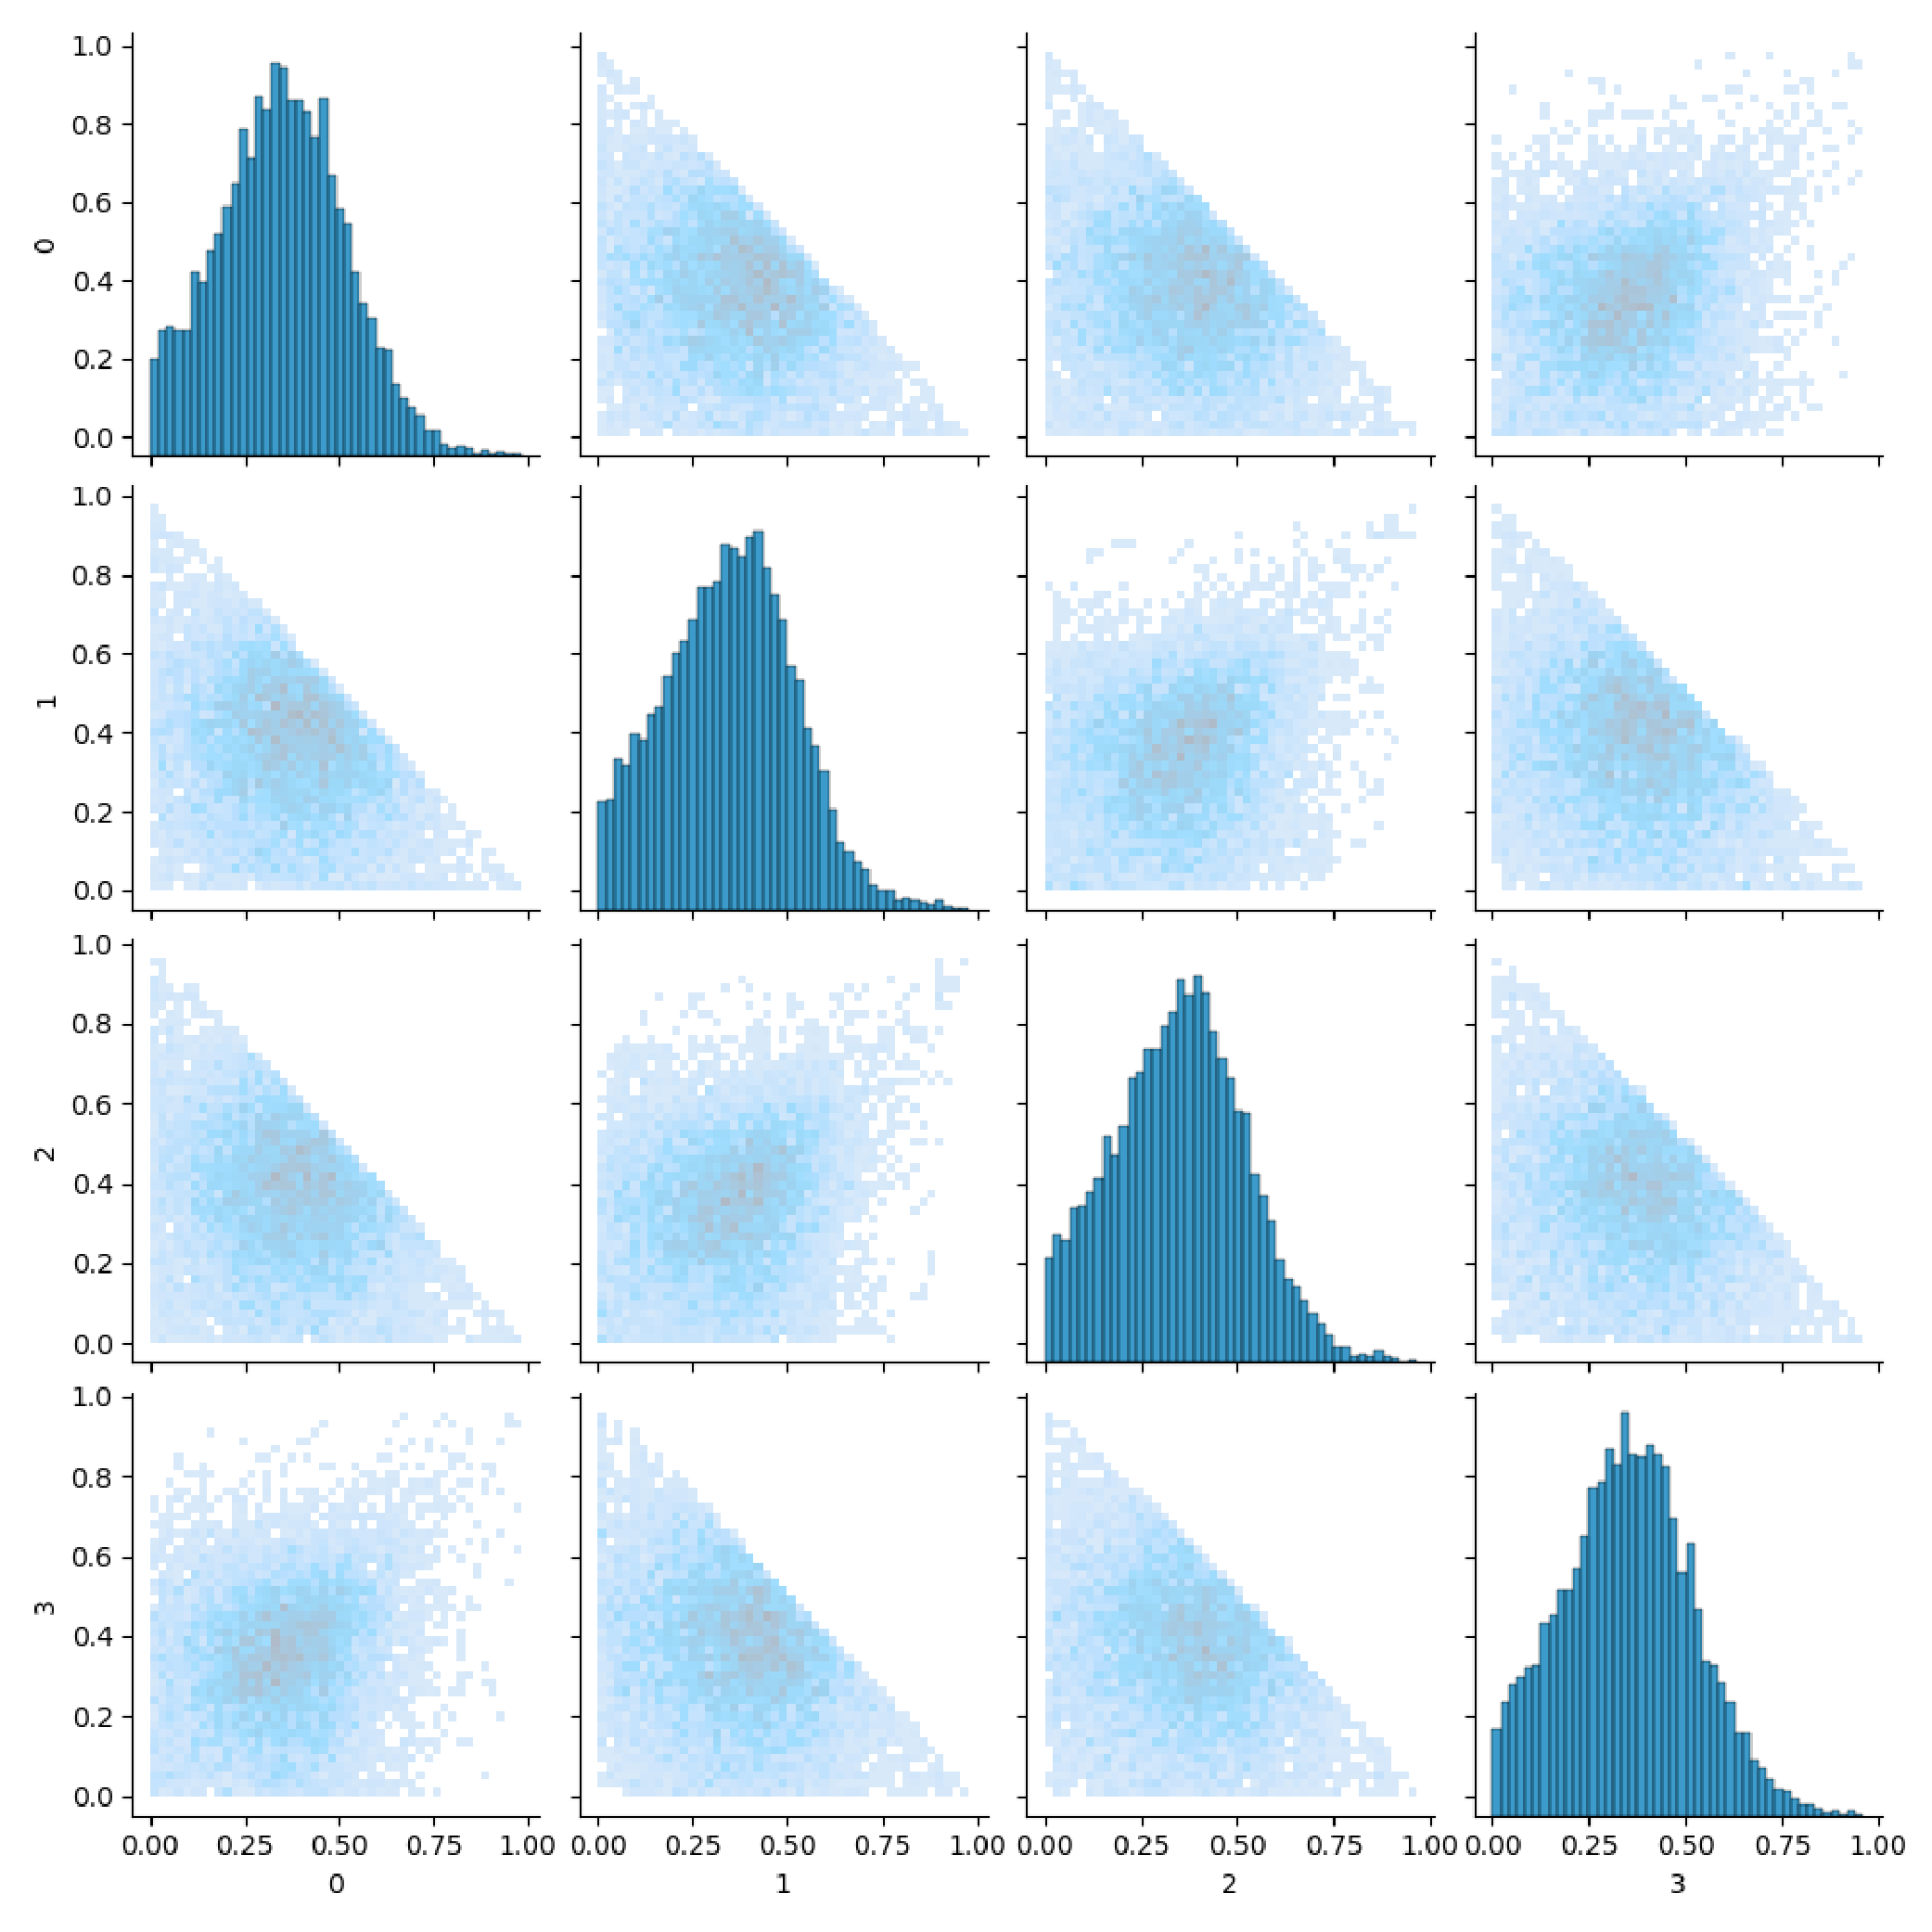
\includegraphics[width=\linewidth]{images/constrained_diffusion/birkhoff_barrier.pdf}
		\caption{Log-barrier.}
		\label{fig:birkhoff_barrier}
	\end{subfigure}
	\hfill
	\begin{subfigure}{0.3\textwidth}
		\centering
		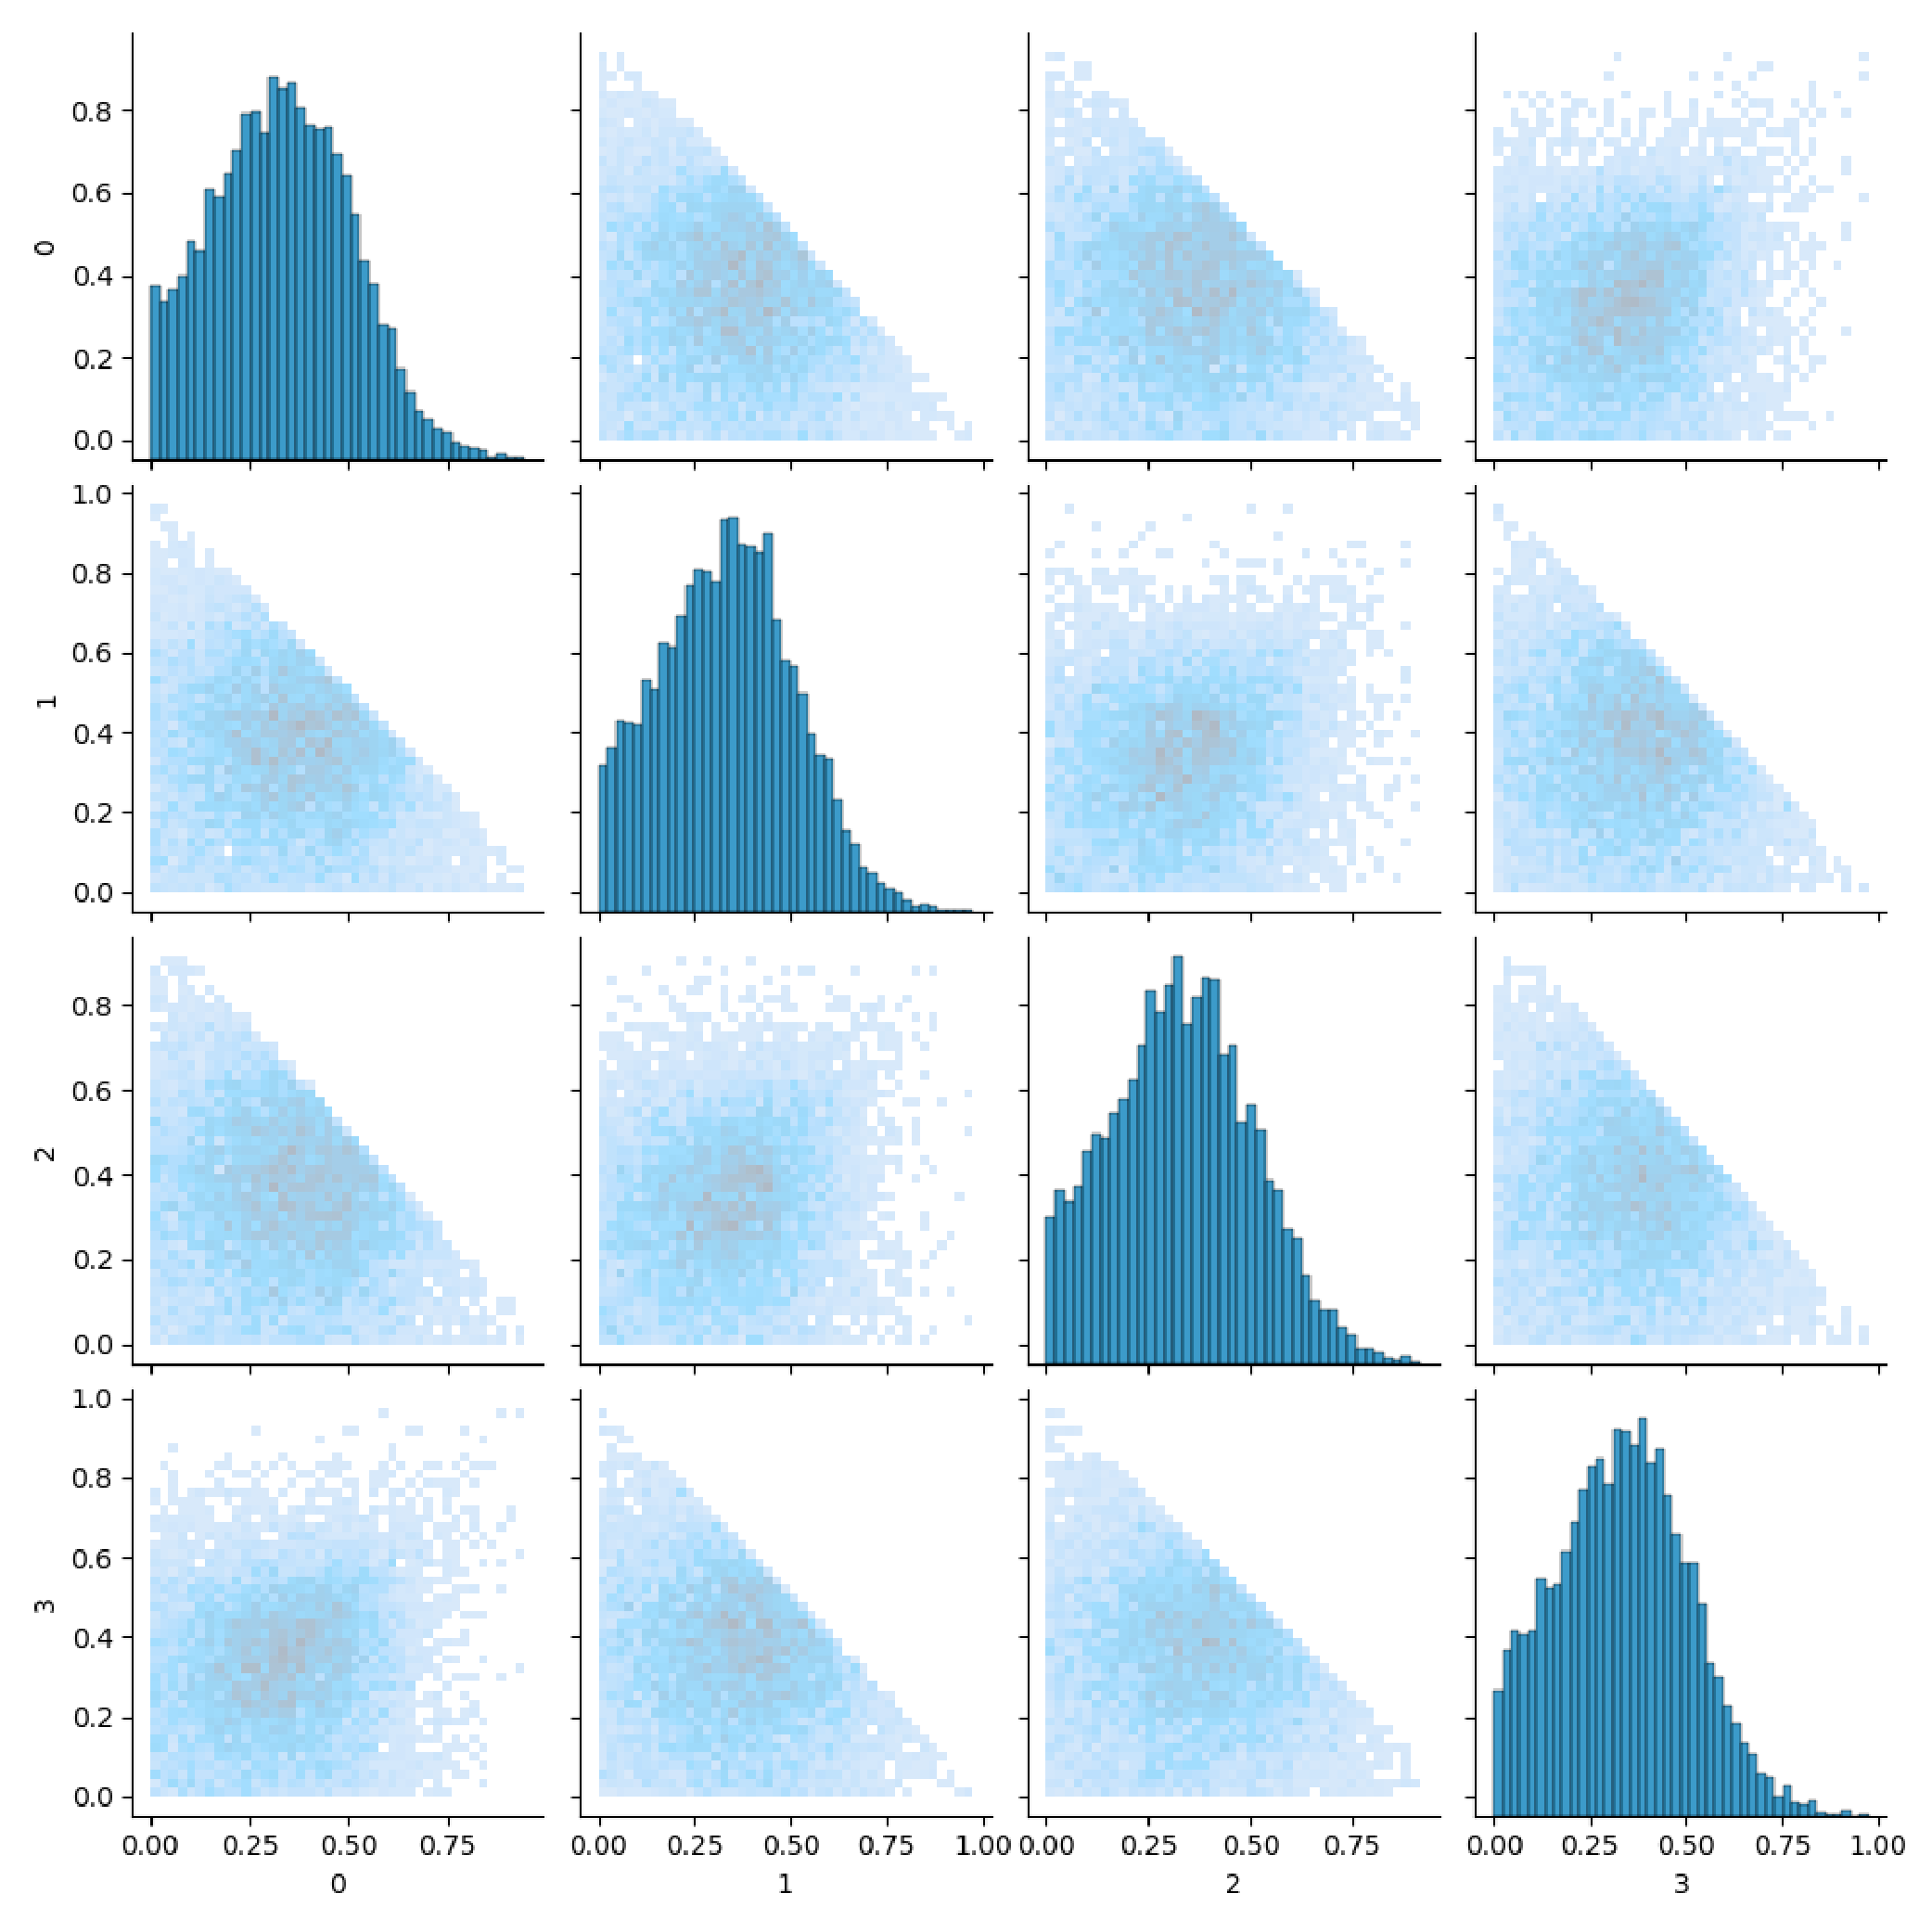
\includegraphics[width=\linewidth]{images/constrained_diffusion/birkhoff_reflected.pdf}
		\caption{Reflected.}
		\label{fig:birkhoff_reflected}
	\end{subfigure}
	\caption{Pairwise and marginals samples on the Birkhoff polytope from synthetic data distribution and from trained constrained diffusion models.}
	\label{fig:birkhoff}
\end{figure}

\subsection{Constrained SPD matrices for robotic arms modelling}
\label{sec:app_spd_exp}

\begin{figure}[H]
	\centering
	\begin{subfigure}{0.27\textwidth}
		\centering
		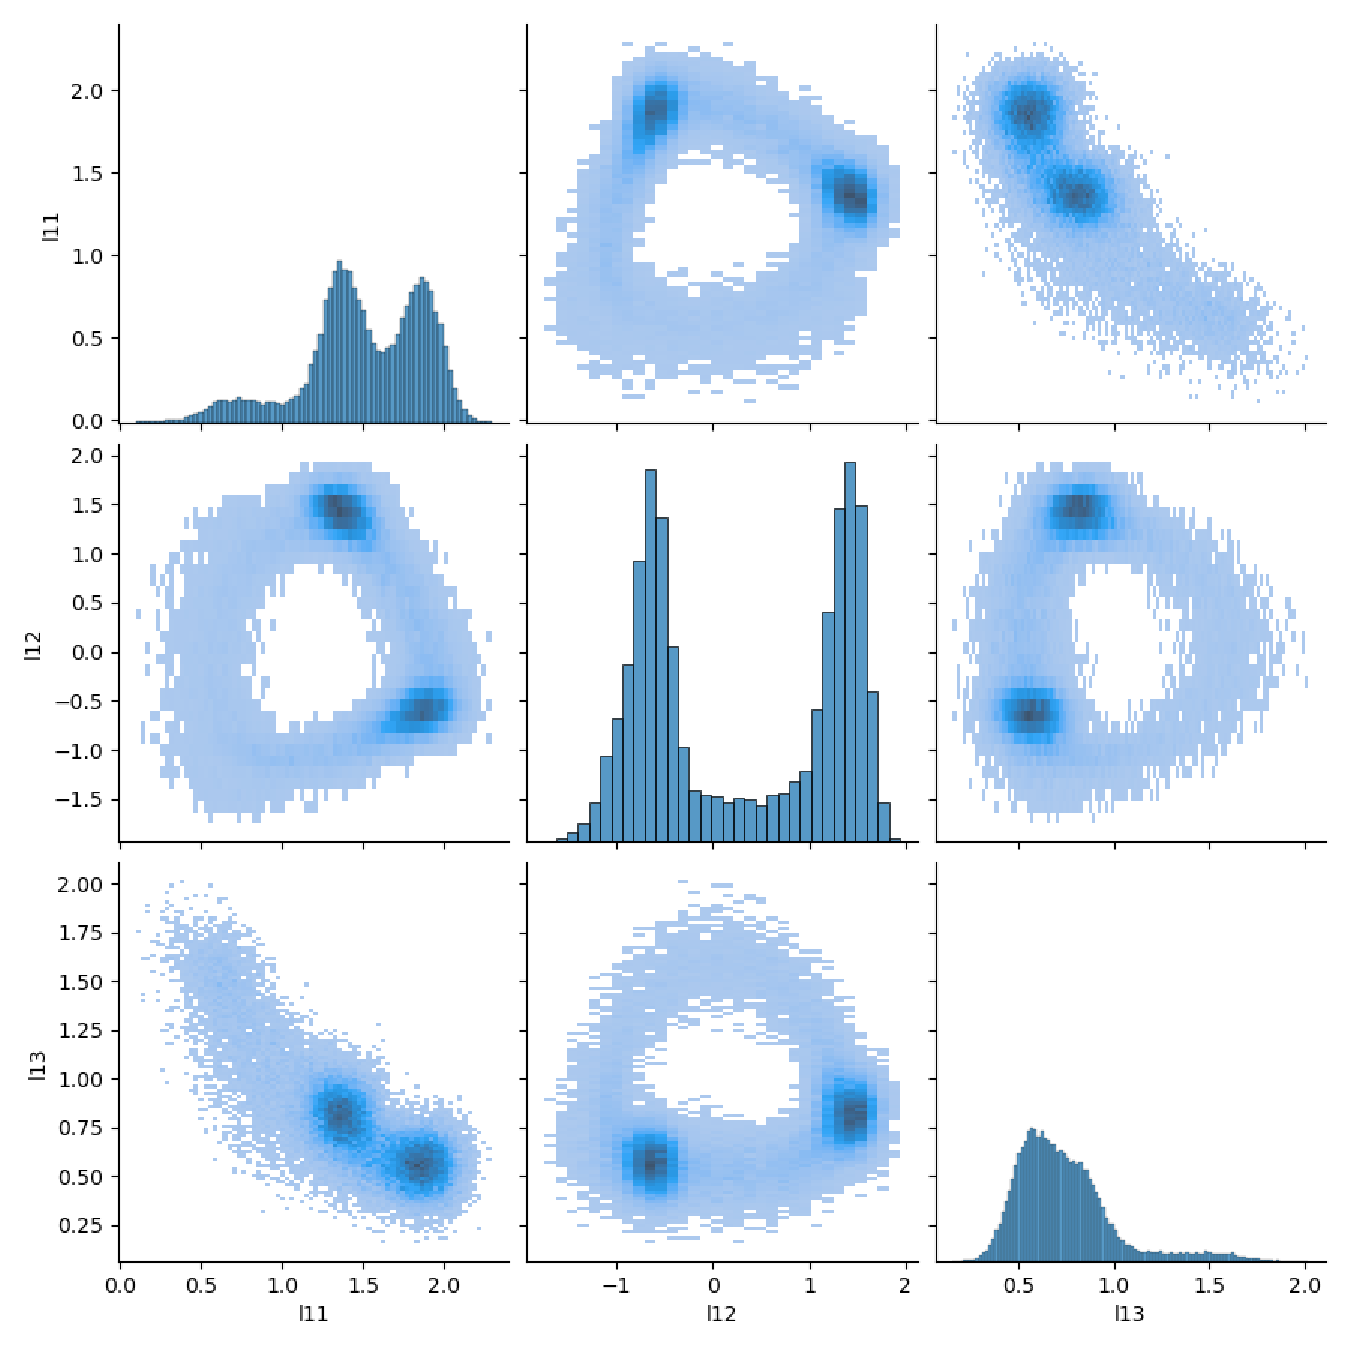
\includegraphics[width=\linewidth]{images/constrained_diffusion/spd_data_ll.pdf}
		\caption{Data.}
		\label{fig:spd_ll_data}
	\end{subfigure}
	\hfill
	\begin{subfigure}{0.27\textwidth}
		\centering
		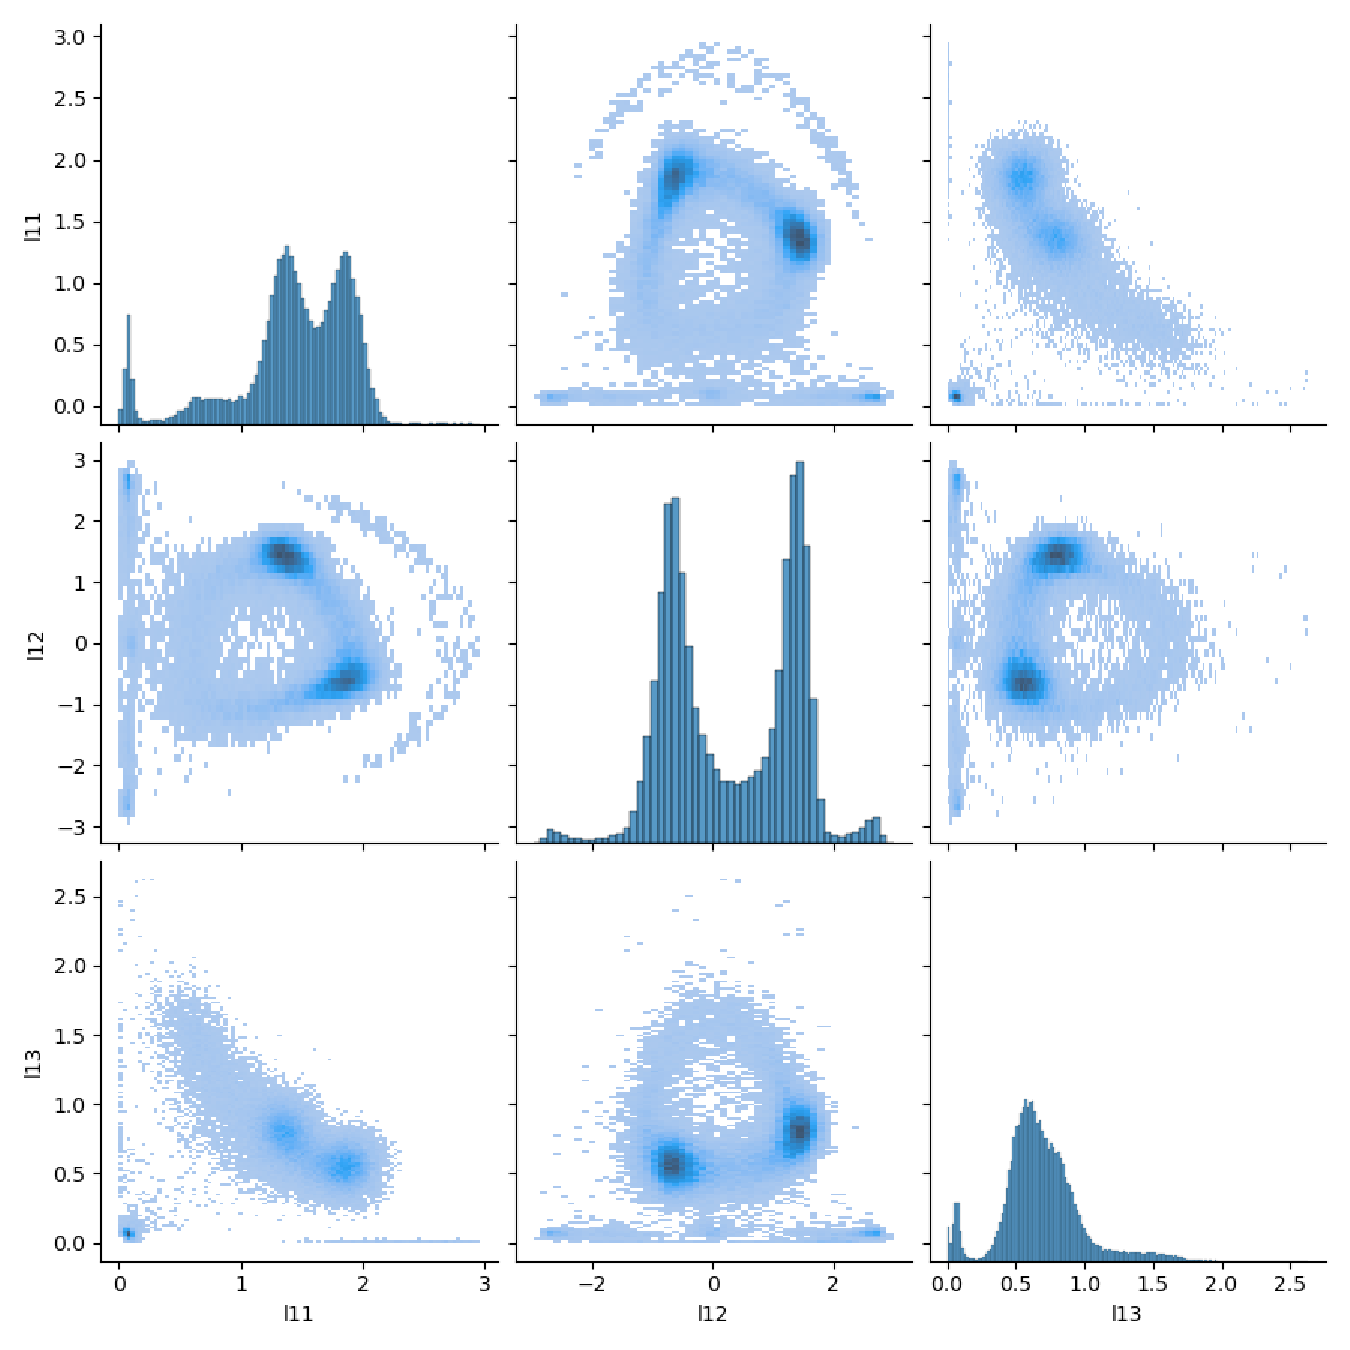
\includegraphics[width=\linewidth]{images/constrained_diffusion/spd_logbarrier_ll.pdf}
		\caption{Log-barrier.}
		\label{fig:spd_ll_barrier}
	\end{subfigure}
	\hfill
	\begin{subfigure}{0.27\textwidth}
		\centering
		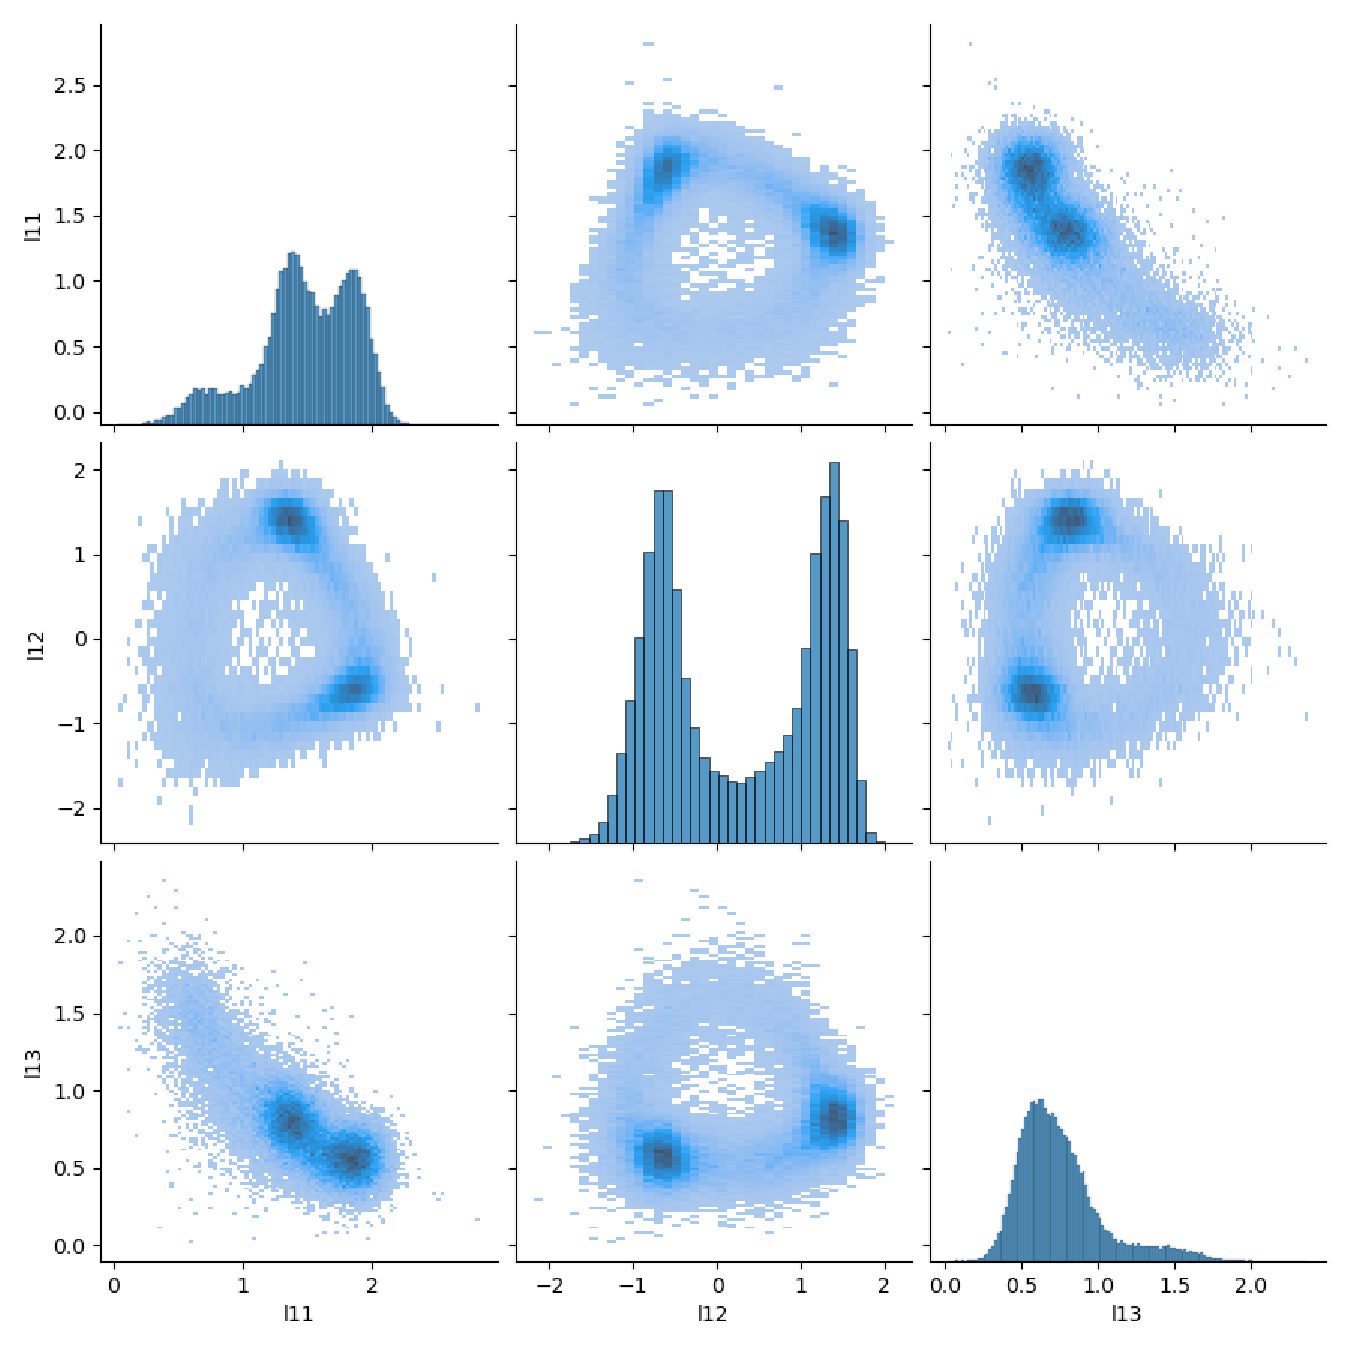
\includegraphics[width=\linewidth]{images/constrained_diffusion/spd_reflected_ll.pdf}
		\caption{Reflected.}
		\label{fig:spd_ll_reflected}
	\end{subfigure}
	\caption{
		Pairwise and marginals distributions over the coefficients \(\mathrm{L}_{11}, \mathrm{L}_{21}, \mathrm{L}_{22}\) of the lower triangle matrix parametrising SPD matrices \(\mathrm{M} = \mathrm{L} \mathrm{L}^\top\) (which represent the manipulability ellipsoids of the robotic arms).
	}
	\label{fig:spd}
\end{figure}

\begin{figure}[H]
	\centering
	\begin{subfigure}{0.27\textwidth}
		\centering
		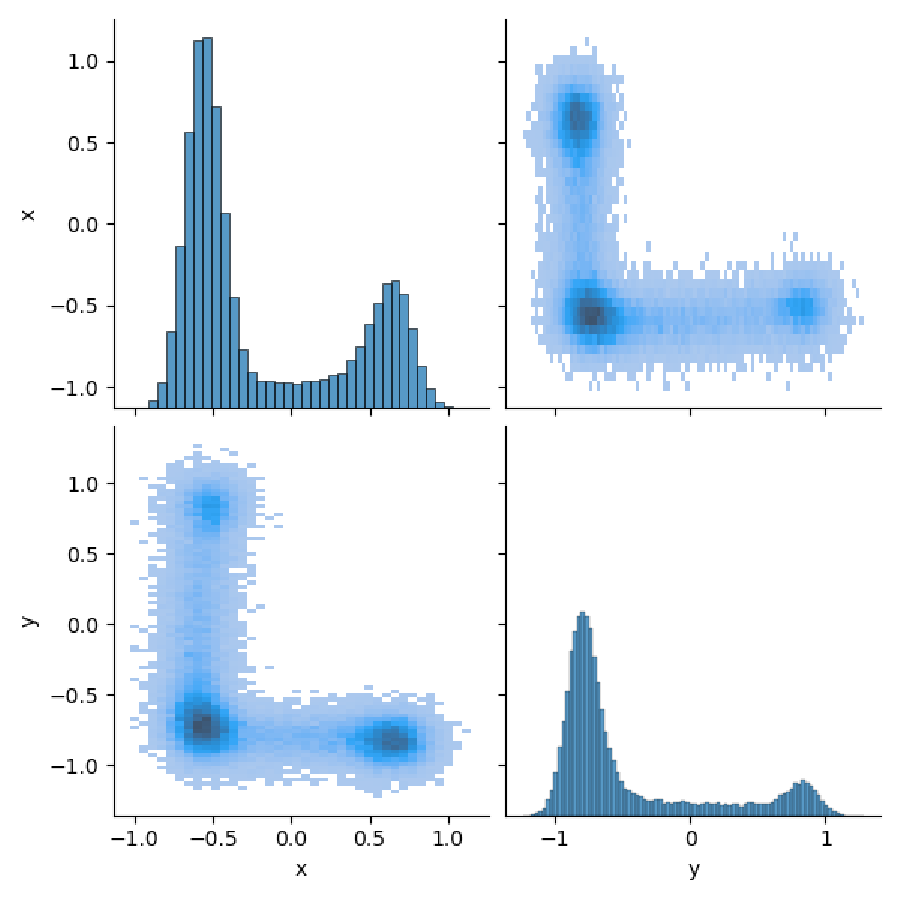
\includegraphics[width=\linewidth]{images/constrained_diffusion/spd_data_xy.pdf}
		\caption{Data.}
		\label{fig:spd_xy_data}
	\end{subfigure}
	\hfill
	\begin{subfigure}{0.27\textwidth}
		\centering
		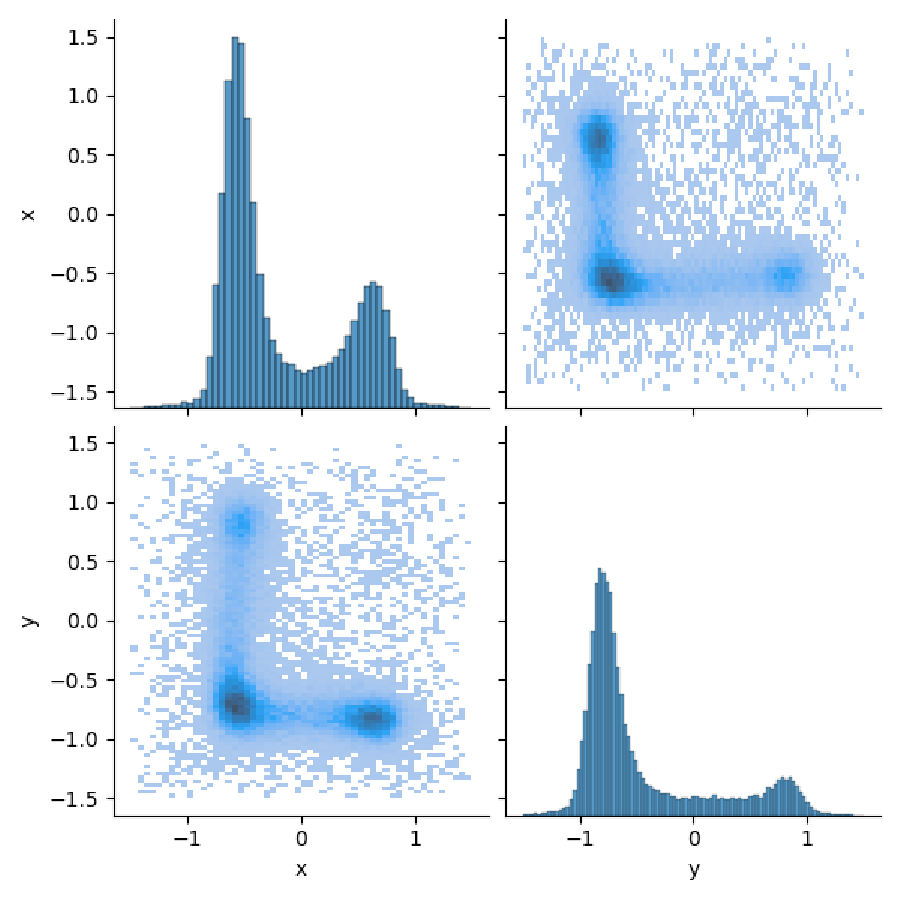
\includegraphics[width=\linewidth]{images/constrained_diffusion/spd_logbarrier_xy.pdf}
		\caption{Log-barrier.}
		\label{fig:spd_xy_barrier}
	\end{subfigure}
	\hfill
	\begin{subfigure}{0.27\textwidth}
		\centering
		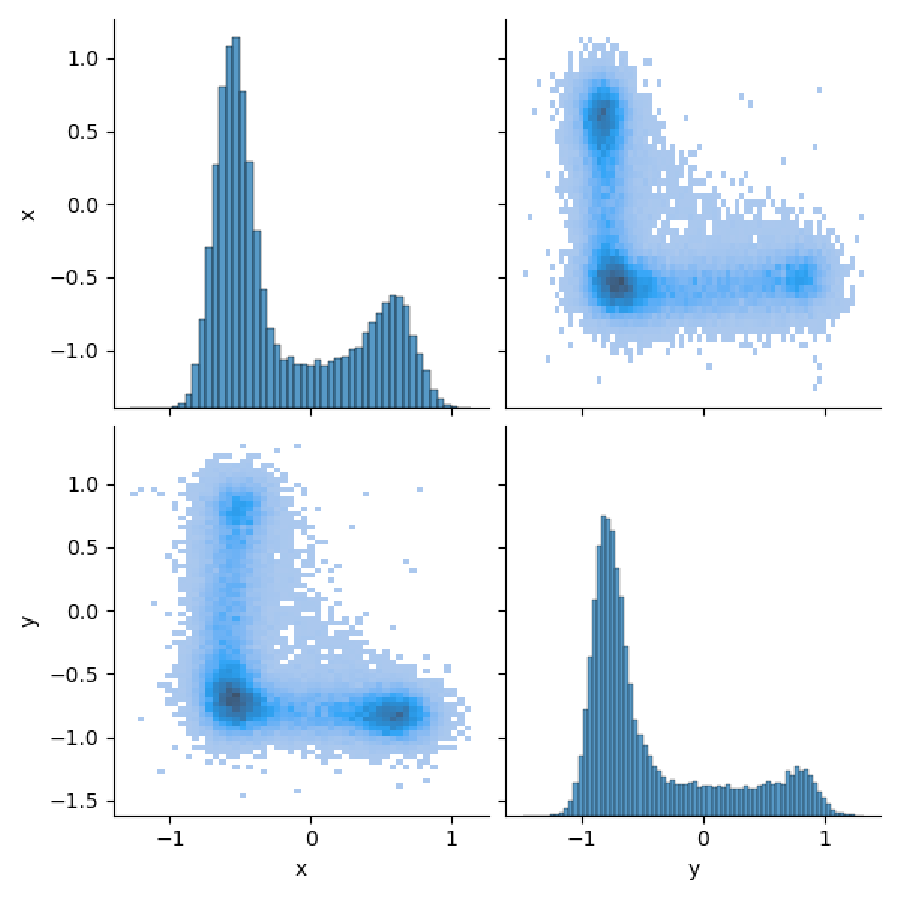
\includegraphics[width=\linewidth]{images/constrained_diffusion/spd_reflected_xy.pdf}
		\caption{Reflected.}
		\label{fig:spd_xy_reflected}
	\end{subfigure}
	\caption{
		Pairwise and marginals distributions over the \((x,y)\) locations of the robotic arms.
	}
	\label{fig:spd_dupref}
\end{figure}

\subsection{Conformational modelling of polypeptide backbones under anchor point constraints}
\label{sec:app_protein_exp}

\begin{figure}[h]
	\centering
	\begin{subfigure}{0.3\textwidth}
		\centering
		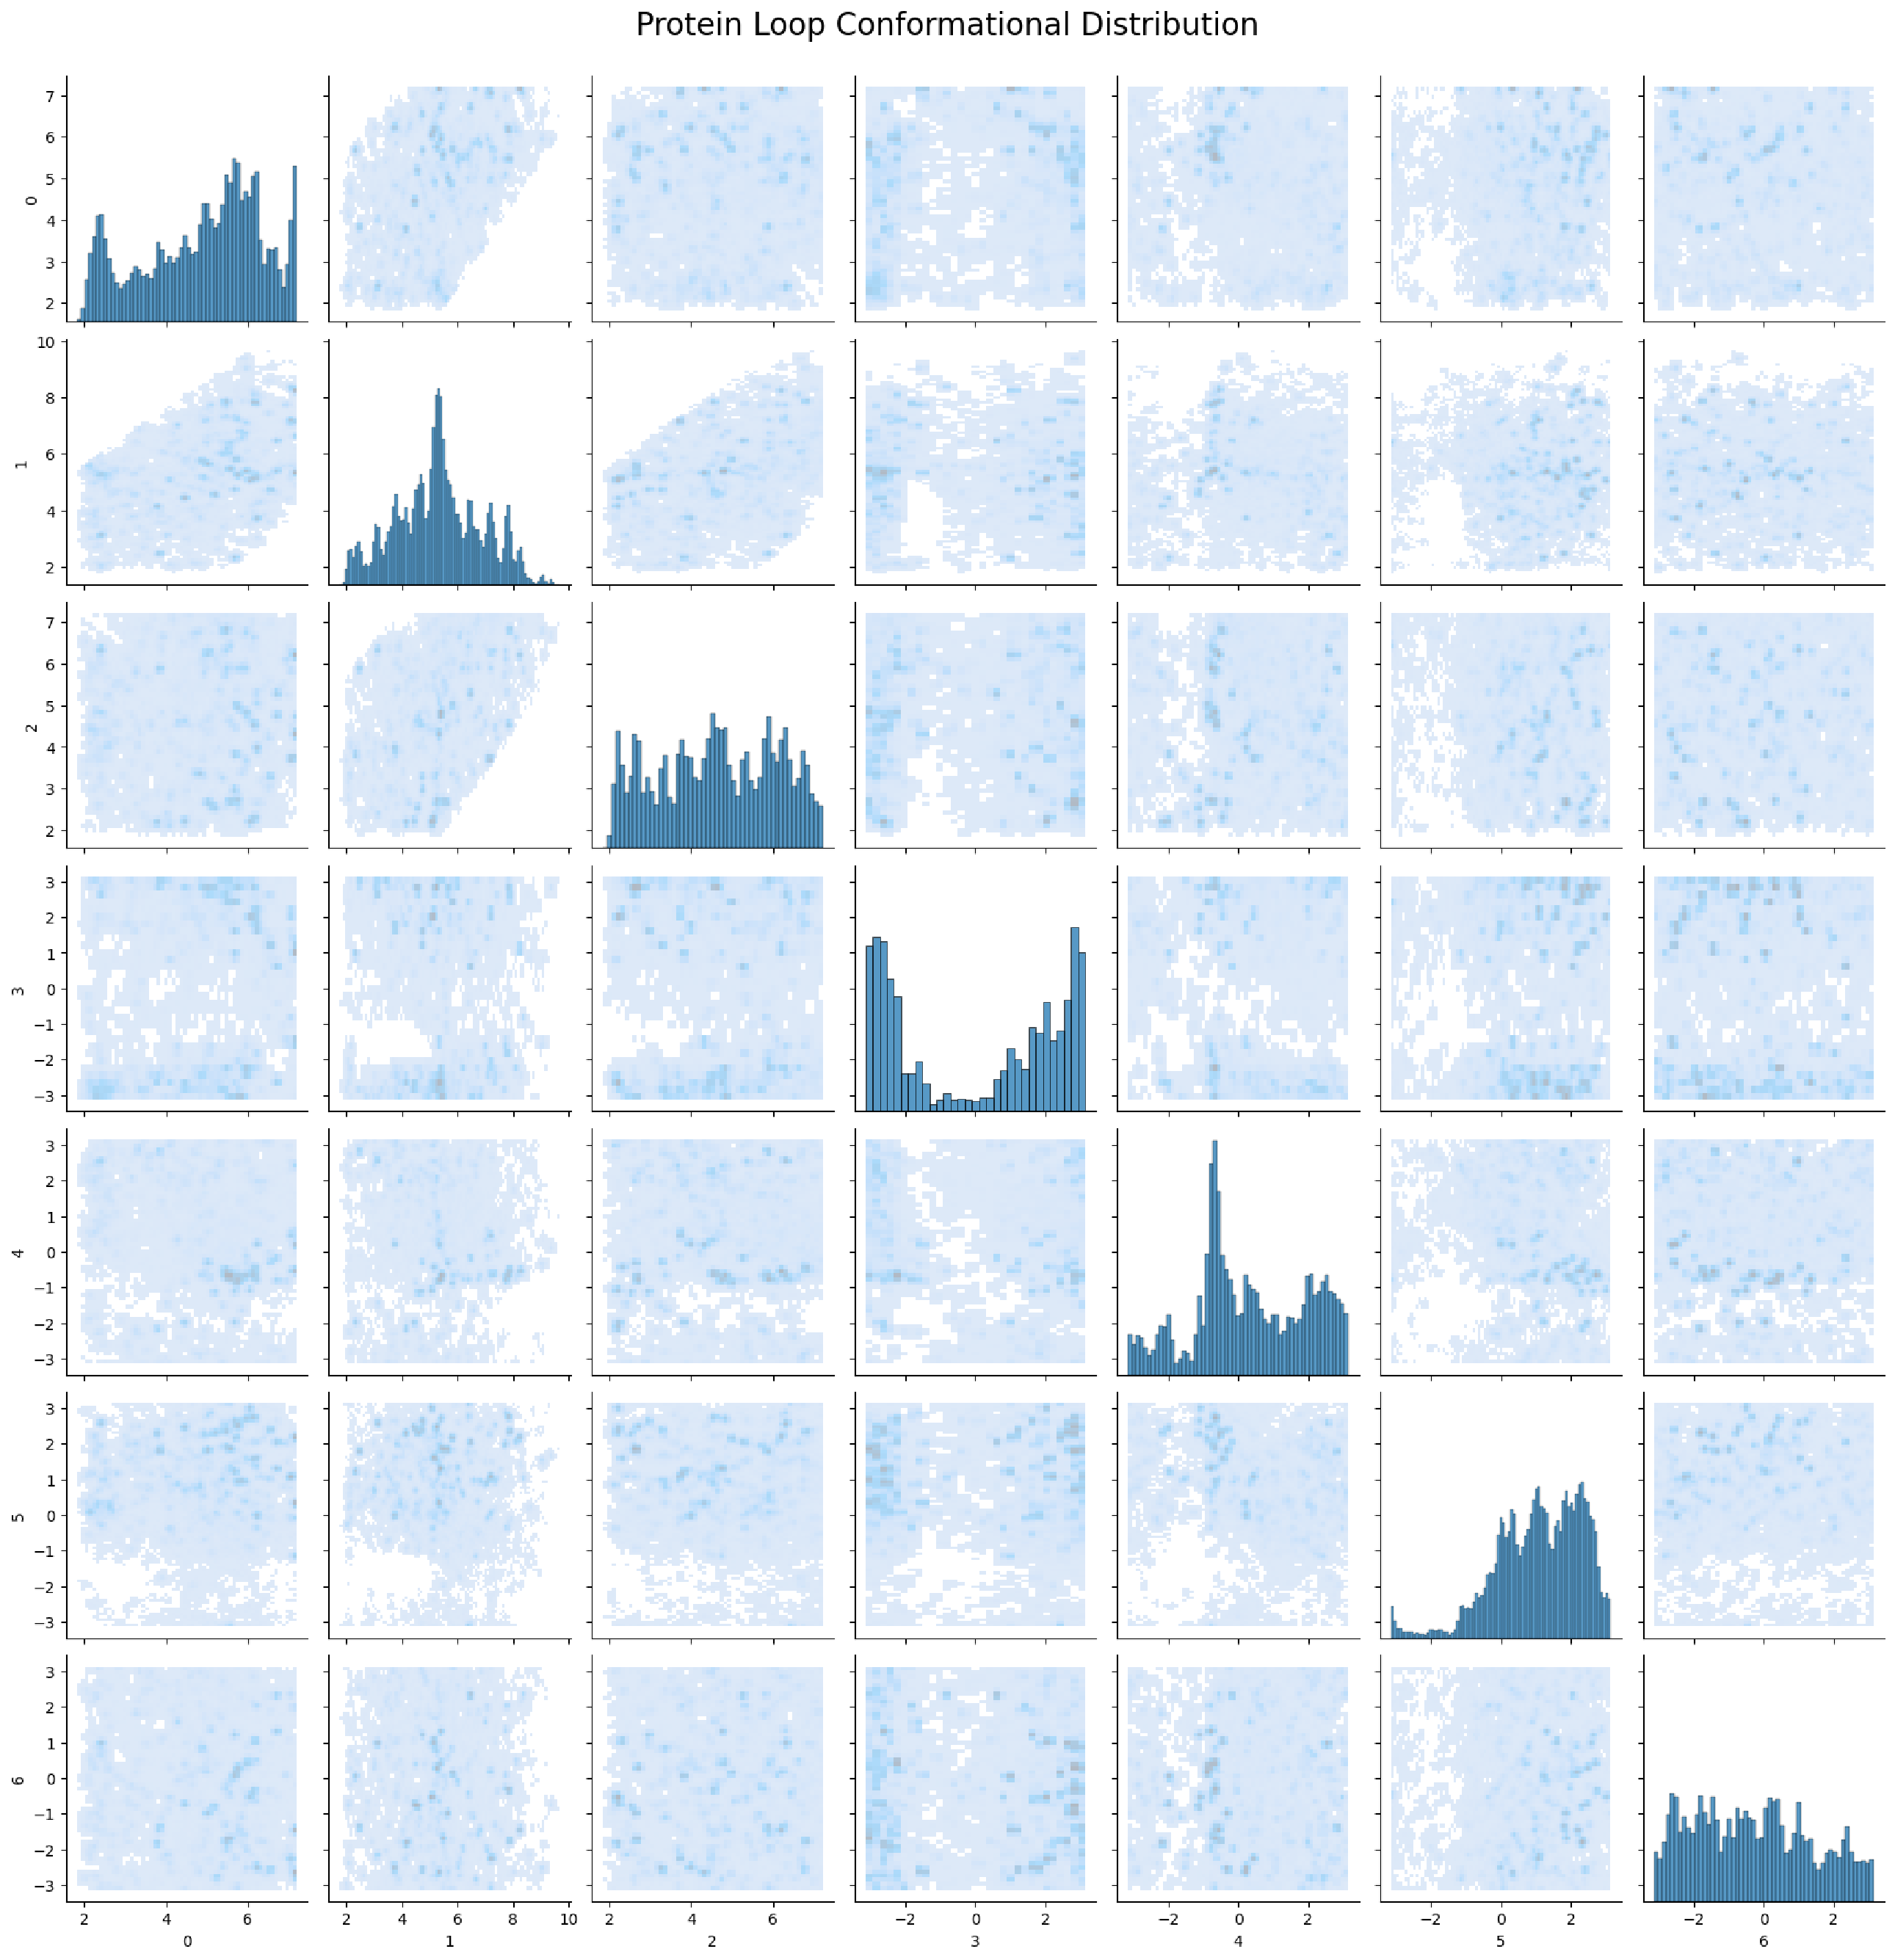
\includegraphics[width=\linewidth]{images/constrained_diffusion/real_loops.pdf}
		\caption{Data.}
	\end{subfigure}
	\hfill
	\begin{subfigure}{0.3\textwidth}
		\centering
		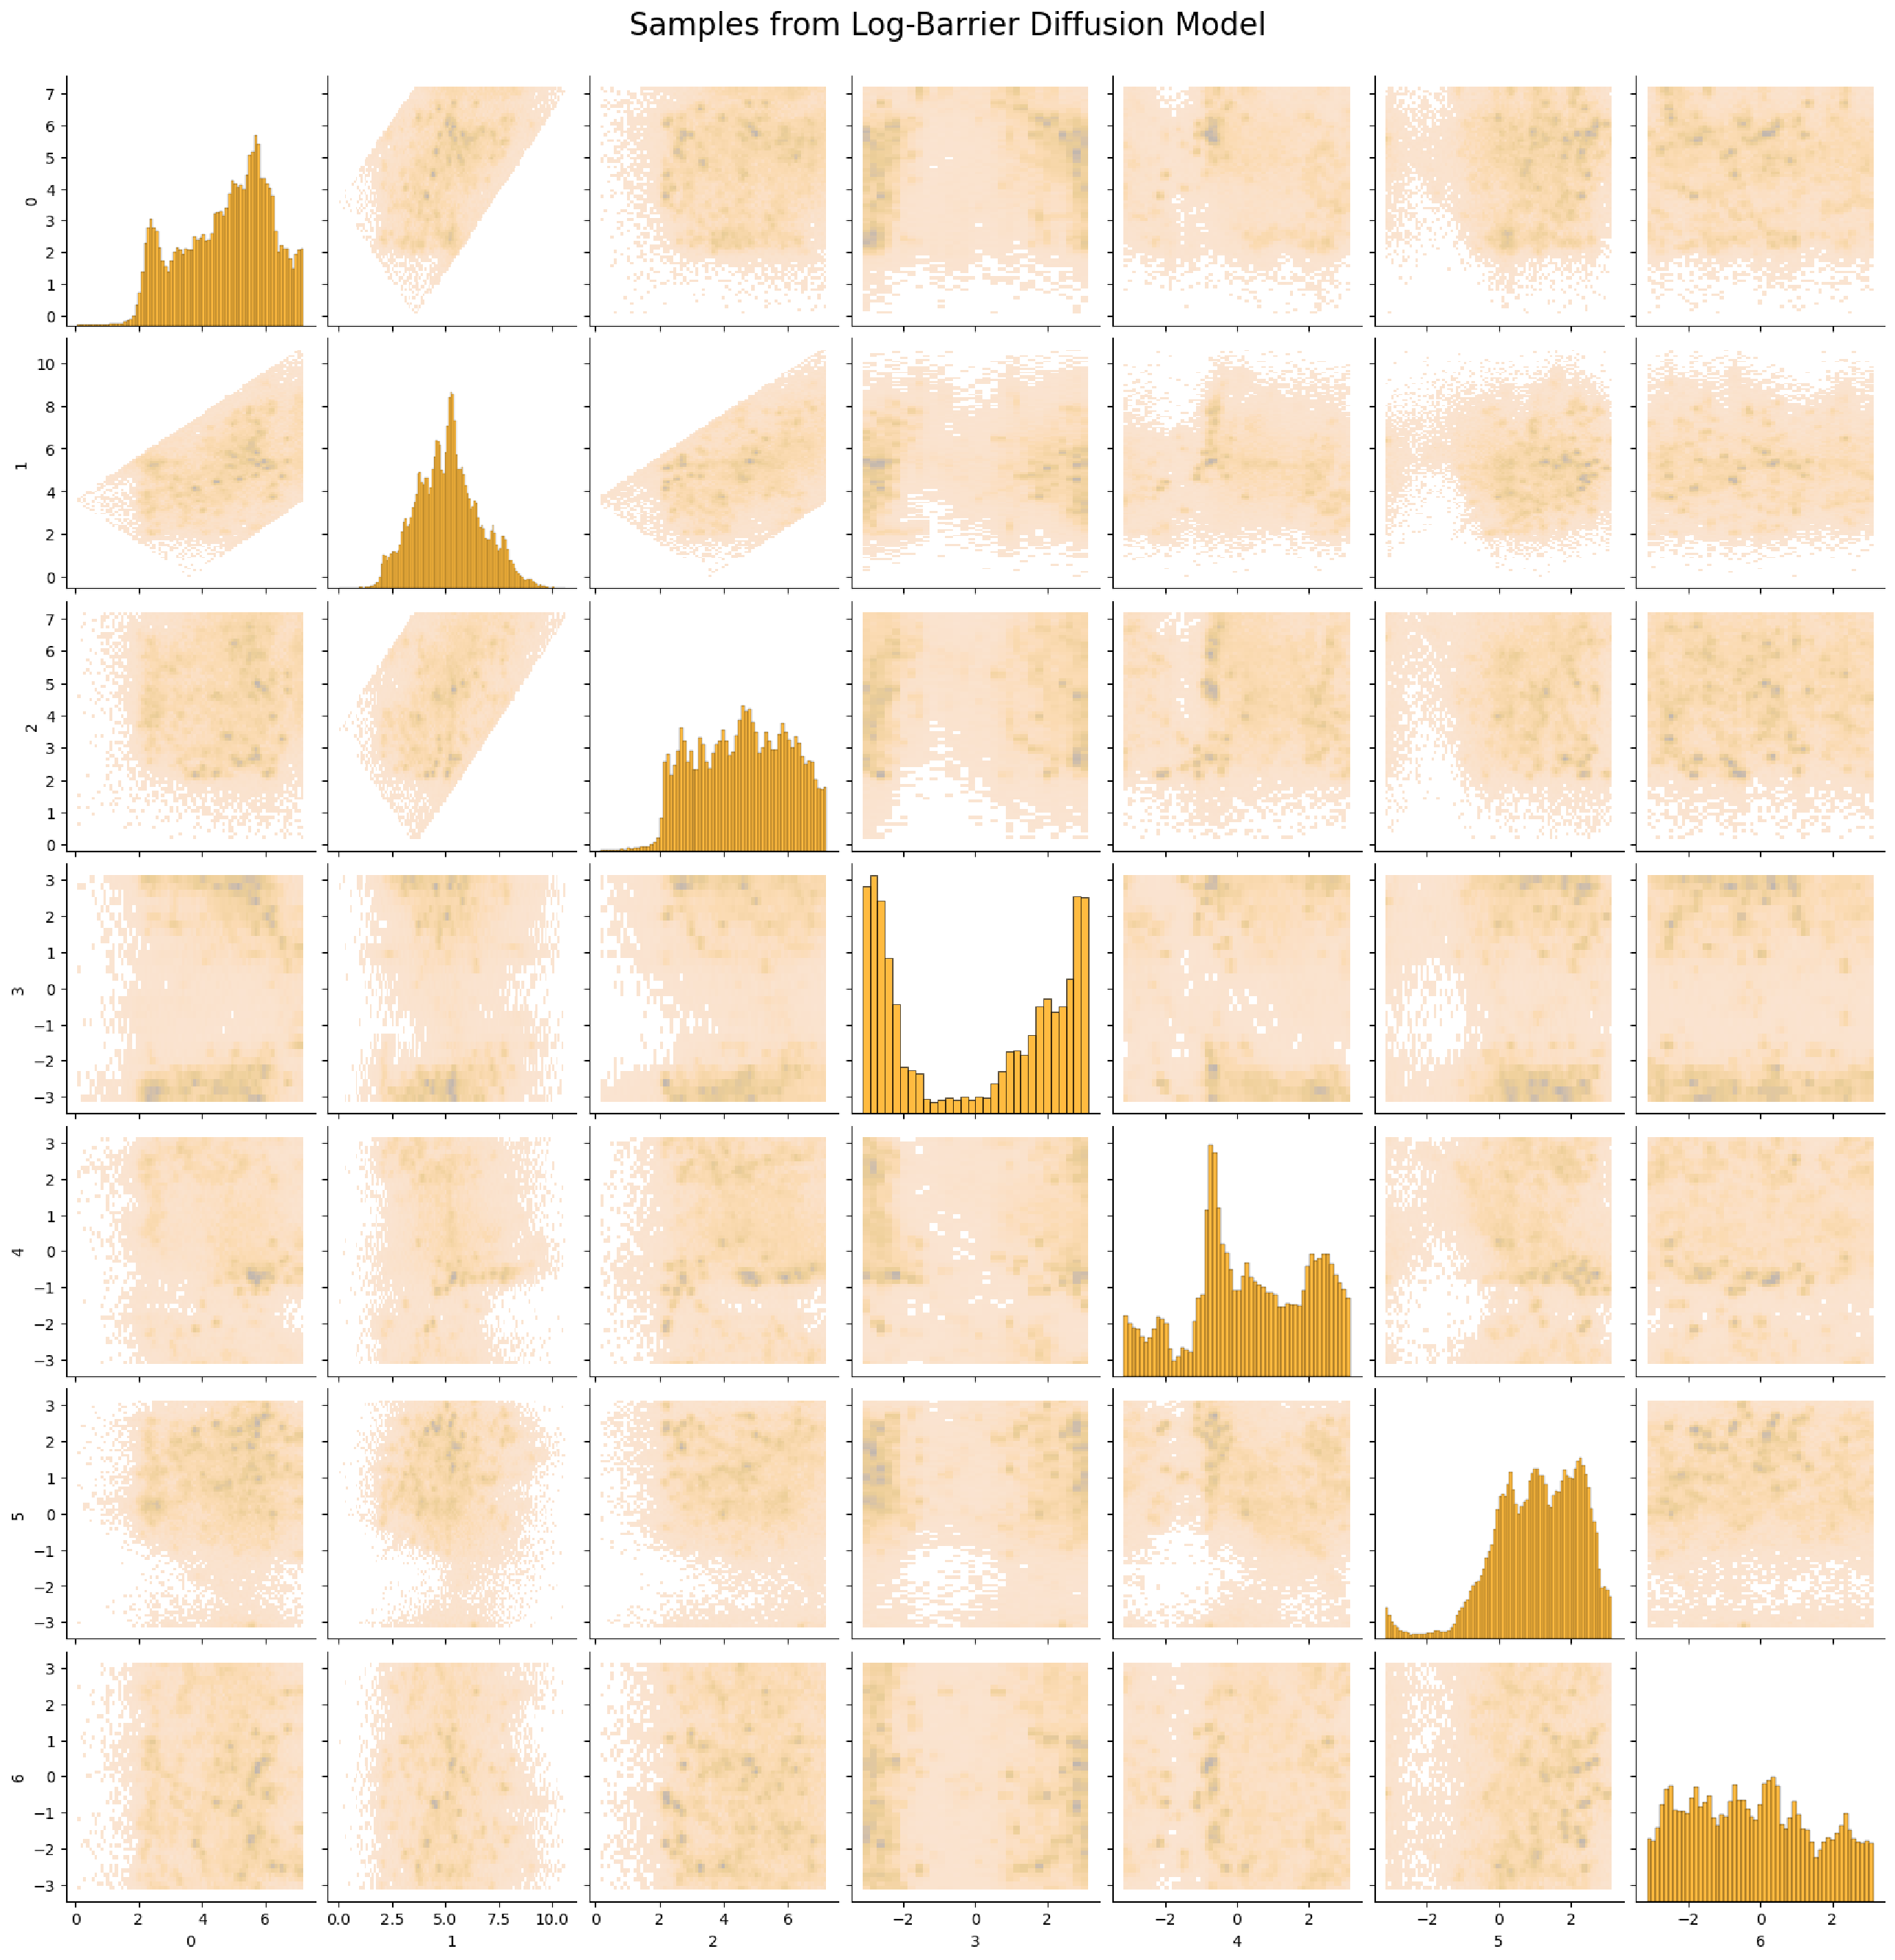
\includegraphics[width=\linewidth]{images/constrained_diffusion/log_loops.pdf}
		\caption{Log-barrier.}
		\label{fig:loops_log}
	\end{subfigure}
	\hfill
	\begin{subfigure}{0.3\textwidth}
		\centering
		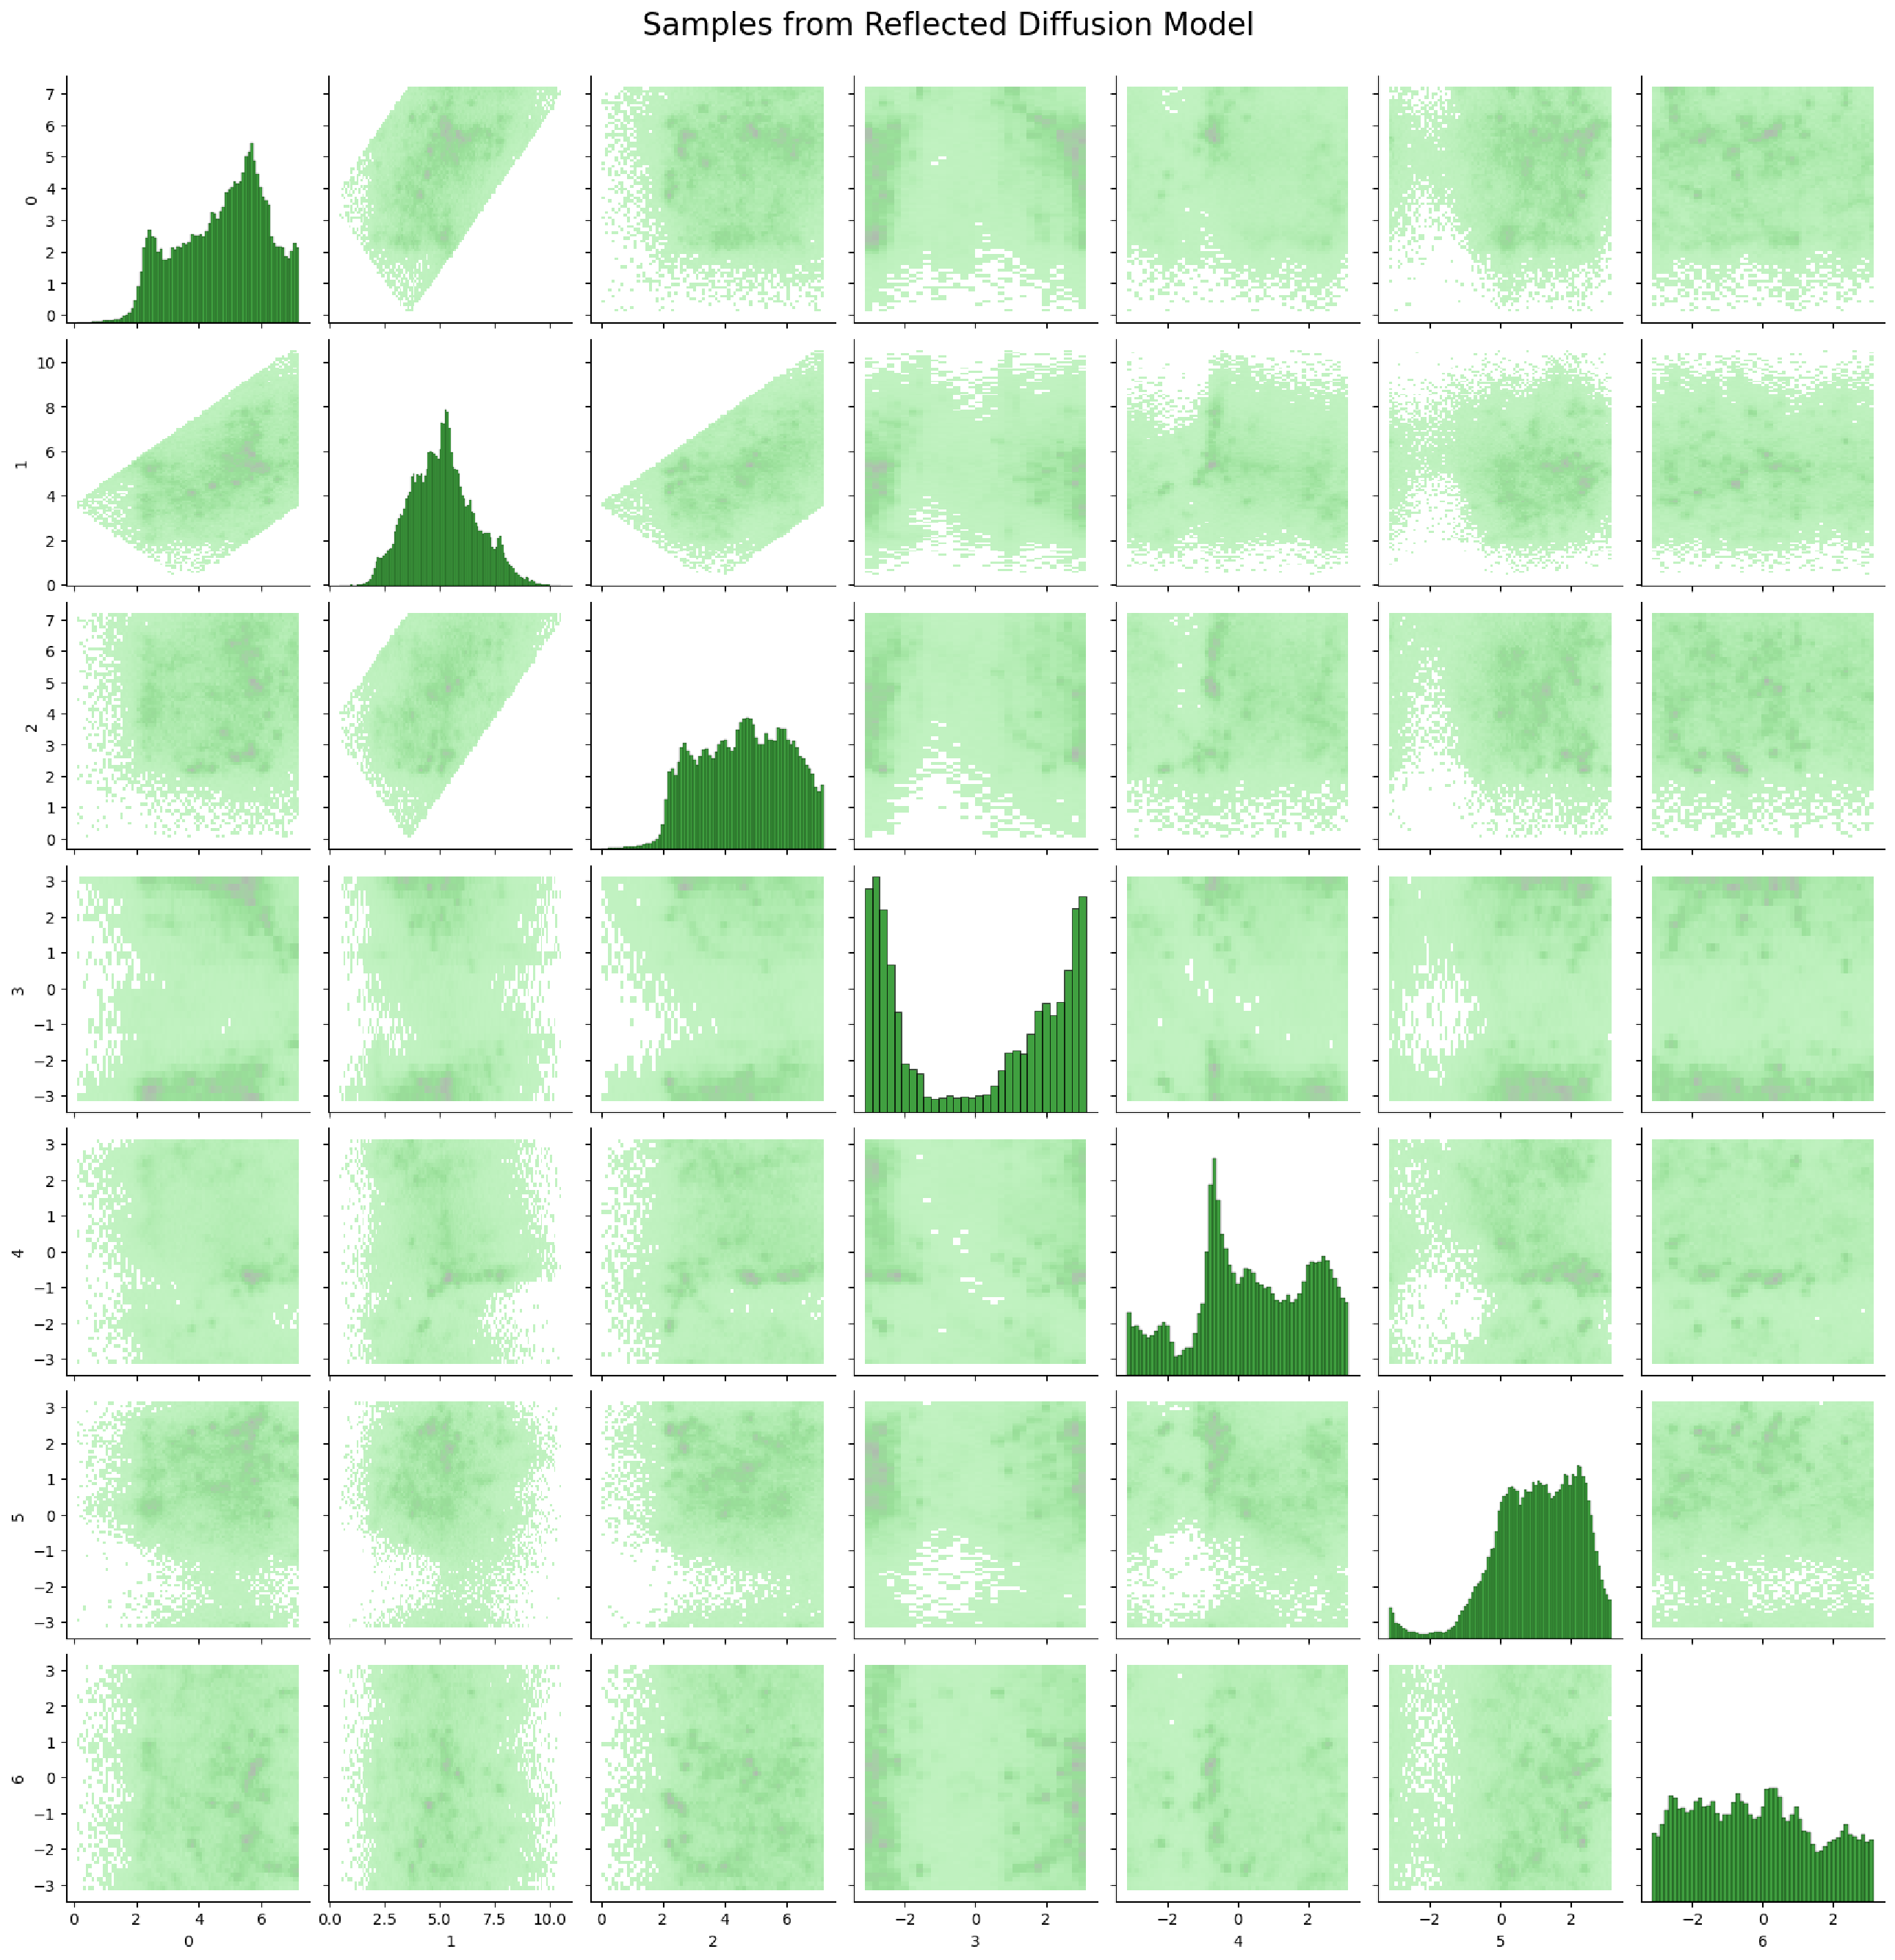
\includegraphics[width=\linewidth]{images/constrained_diffusion/reflected_loops.pdf}
		\caption{Reflected.}
		\label{fig:loops_reflected}
	\end{subfigure}
	\caption{
		Pairwise and marginals distributions over the dimensions of the polytope and torus used to model the conformational ensembles of cyclic peptides generated by the reflected diffusion model.
	}
	\label{fig:loops_pairs}
\end{figure}
